% !TeX root = main
\documentclass[a4paper, 11pt]{article}

%------------------------------------------------------------------------------------
% import packages
\usepackage[scaled]{helvet}
%\usepackage{courier}
%\renewcommand\familydefault{\sfdefault} 

% Should include times new roman according to the slides
\usepackage{mathptmx}

% To use matrix
\usepackage{amsmath}

% To use mathbb
\usepackage{amssymb}

% To draw FSA
\usepackage{tikz}
\usetikzlibrary{automata,positioning,decorations.text,topaths,arrows.meta,decorations.pathmorphing,quotes}

\usepackage[T1]{fontenc}
\usepackage[english]{babel}
\usepackage{graphicx}
\usepackage{tabularx}
\usepackage{ltablex}
\usepackage{multirow}
\usepackage{subfig}
\usepackage{caption, booktabs}
\usepackage[hidelinks]{hyperref}
\usepackage[shortlabels]{enumitem}

% Font weight for pictures labels
\usepackage[labelfont=bf]{caption}

% No indent on new paragraphs
\usepackage[parfill]{parskip}

% Margins
\usepackage[margin=1in]{geometry}

% Set TOC Depth
\setcounter{tocdepth}{3}

% Left space
\usepackage{scrextend}

% Matrix with more than 10 columns
\setcounter{MaxMatrixCols}{20}

% code
\usepackage{listings}
\usepackage{color}
\definecolor{lightgray}{rgb}{.9,.9,.9}
\definecolor{darkgray}{rgb}{.4,.4,.4}
\definecolor{purple}{rgb}{0.65, 0.12, 0.82}
\lstdefinelanguage{Matlab}{
  keywords={typeof, new, true, false, catch, function, return, null, catch, switch, var, if, in, while, do, else, case, break, all},
  keywordstyle=\color{blue}\bfseries,
  ndkeywords={class, export, boolean, throw, implements, import, this},
  ndkeywordstyle=\color{darkgray}\bfseries,
  identifierstyle=\color{black},
  sensitive=false,
  comment=[l]{\%},
  morecomment=[s]{/*}{*/},
  commentstyle=\color{orange}\ttfamily,
  stringstyle=\color{red}\ttfamily,
  morestring=[b]',
  morestring=[b]"
}

\lstset{
    language=Matlab,
    extendedchars=true,
    basicstyle=\footnotesize\ttfamily,
    showstringspaces=false,
    showspaces=false,
    %numbers=left,
    numberstyle=\footnotesize,
    numbersep=9pt,
    tabsize=2,
    breaklines=true,
    showtabs=false,
    captionpos=b,
    breaklines=true,
    morekeywords={matlab2tikz},
    keywordstyle=\color{blue},
    morekeywords=[2]{1}, keywordstyle=[2]{\color{black}},
    identifierstyle=\color{black},
    stringstyle=\color{mylilas},
    commentstyle=\color{mygreen},
    showstringspaces=false,%without this there will be a symbol in the places where there is a space
    %emph=[1]{for,end,break},emphstyle=[1]\color{red},
    emph=[1]{for,end,break},emphstyle=[1]\color{blue},
    frame=single
}

% functions with arrow
\newcommand{\f}[2]{\ensuremath{f:\,\,{#1}\rightarrow {#2}}}

% brackets
\newcommand{\brackets}[1]{\ensuremath{\{{#1}\}}}
\newcommand{\Brackets}[1]{\ensuremath{\begin{Bmatrix}
    {#1}
\end{Bmatrix}}}

% insieme quoziente
\newcommand{\bigslant}[2]{{\raisebox{.2em}{$#1$}\left/\raisebox{-.2em}{$#2$}\right.}}

% underlabel
\newcommand{\underlabel}[2]{\ensuremath{
    \underset{\text{#2}}{\underbrace{#1}}
}}

% mybox
\newcommand{\mybox}[1]{
    \fbox{\begin{minipage}{\linewidth}
        \vspace{1em}
        #1
        \vspace{1em}
    \end{minipage}}
}

\graphicspath{ {images/} }
\hypersetup{
    colorlinks,
    citecolor=black,
    filecolor=black,
    linkcolor=black,
    urlcolor=black
}

\begin{document}

\begin{titlepage}
	\centering
    \begin{tabular}{rl}
        Alessio Hu & (12345678)
    \end{tabular}

    \vspace{1.5cm}
    {\Huge \textbf{Multimedia Signals Processing\\}}
    \vspace{1.5cm}
    {\large 
        Multimedia Signals Processing \\
        Prof. Marco Marcon \\ 
		DEIB - Politecnico di Milano \par
    }
    \vspace{1.5cm}
    {\large \textbf{Something:}\\
    \vspace{0.5cm}
    Something else}
    \par
    \vspace{3cm}
    
\includegraphics[scale=0.4]{images/logo.pdf}
    \par
    \vspace{3cm}
	A.Y. 2022-2023
\end{titlepage}

\tableofcontents
    % !TeX root = ../main.tex

\section{Discrete Signals}
\subsection{Impulse}
    $$
    \delta[n]=\begin{cases}
        1,\text{ $n=0$}\\
        0,\text{ $n\neq0$}
    \end{cases}
    $$

\subsection{Discrete unit step}
    $$
    u[n]=\begin{cases}
        1,\text{ $n\geq0$}\\
        0,\text{ $n<0$}
    \end{cases}
    $$

\subsection{Discrete exponential step}
    $$
    x(n)=a^nu(n)
    $$

\subsection{Discrete periodic signals}
    $$
    x(n)=x(n+kT)\qquad\forall\,\,k\in\,\,\mathbb{Z}
    $$

\subsection{Discrete-time sinusoids}
From continuous to discrete
    $$
    y(t)=A\cdot\cos(2\pi f_0t+\phi)\rightarrow y(n)=A\cdot\cos(2\pi f_0T_sn+\phi)
    $$
    \begin{center}
        OR
    \end{center}
    $$
    \begin{cases}
        y(t)=A\cdot\cos(2\pi f_0t+\phi)\rightarrow y(n)=A\cdot\cos(2\pi \tilde{f_0}n+\phi)\\
        \tilde{f_0}=\frac{f_0}{F_s}=f_0\cdot T_s\qquad\text{ normalized frequency}\\
        \tilde{\omega_0}=2\pi\tilde{f_0}=\frac{\omega_0}{F_s}=\omega_0T_s
    \end{cases}
    $$
\begin{itemize}
    \item $A=$ amplitude
    \item $f_0=$ frequency [Hz]
    \item $\omega_0=2\pi f_0=$ angular frequency [rad/s]
    \item $\phi=$ phase [rad]
    \item $\frac{1}{f_0}=\frac{2\pi T_s}{\tilde{\omega_0}}=$ \textbf{period of the sinusoid [seconds]}
    \item $P_{samples}=\frac{1}{f_0\cdot T_s}=\frac{1}{\tilde{f_0}}=\frac{2\pi}{\tilde{\omega_0}}=\frac{F_s}{f_0}$ \textbf{period of the sinusoid [in samples]}
    \item $t=n\cdot T_s=\left[start:T_s=\frac{1}{F_s}:end=\frac{1}{f_0}-\frac{1}{F_s}\right]$
    \item $n=0,1,2,\cdots N=$ samples
    \item $T_s=$ sampling time or sampling period
    \item $F_s=\frac{1}{T_s}=$ \textbf{sampling rate/signal duration [Hz]}
    \item \textbf{Signal as sum of sinusoids}
    \begin{itemize}
        \item \textbf{Principle of superposition}
        $$x=\cos(\omega_1t)+\cos(\omega_2t)+\cos(\omega_3t)$$
        \item \textbf{Global sinusoid period [in samples]}: mcm between the sinusoid periods in samples
    \end{itemize}
\end{itemize}
    % !TeX root = ../main.tex

\section{Linear Time-Invariant Systems}
\begin{itemize}
    \item Linearity = input-output realtionship is linear
    \item Time invariance = the output does not depend on the particular time the input is applied:
    $$x(t)\rightarrow y(t)\leftrightarrow x(t-k)\rightarrow y(t-k)$$
    \item The system can be completely characterized by its impulse response $h(t)$
\end{itemize}

The output:
\begin{LARGE}
    $$
    y(n)=x(n)*h(n)=\sum_{k=-\infty}^\infty x(k)h(n-k)
    $$
\end{LARGE}

\subsection{Convolution}
\begin{itemize}
    \item Flip the second term $h(n)\rightarrow h(-k)$
    \item Shift $h$ by adding $n$ (if positive shift to right, if negative to left) $h(n-k)$
    \item For output $y(n)$ sum all contributions of $x(k)$ and the shifted flipped $h$
\end{itemize}
Last step similar to scalar product. \textbf{The length of the convolution is the sum of the two signals-1 (n+m-1) and the support (x-axis from when the signals start to differ from 0) is the sum of the supports until the final support of the two}.

Properties of convolution:
\begin{itemize}
    \item Commutativity
    \item Associativity
    \item Distributivity
    \item Convolution by pulse $x(n)*\delta(n)=x(n)$
    \item Convolution by a shifted pulse $x(n)*\delta(n-k)=x(n-k)$
\end{itemize}

Alternativetely, if $h(n)=h[n]=$sum of various $\delta$, we can apply the distributive property and sum various convolutions by $\delta$!

\subsection{Discrete delay}
$$y(n)=x(n-k)$$
So:
$$y(n)=x(n)*h(n)=x(n)*\delta(n-k)=x(n-k)$$

\subsection{Moving average}
\begin{LARGE}
    $$
    y(n)=\frac{1}{M}\sum_{m=0}^{M-1}x(n-m)
    $$
\end{LARGE}
It is a filter, result of LTI system.

The \textbf{impulse response}:
$$y(n)=\frac{1}{M}\sum_{m=0}^{M-1}x(n)*\delta(n-m)=x(n)*\sum_{m=0}^{M-1}\delta(n-m)\rightarrow \mathbf{\sum_{m=0}^{M-1}\delta(n-m)}$$

\subsection{Cosine signal and generic filter}
We will get another cosine with very same frequency, but modified amplitude and phase. \textbf{Look at the exercise 20181107-1}
    % !TeX root = ../main.tex

\section{Z transform}
\begin{LARGE}
    $$
    X(z)=\sum_{n=-\infty}^{+\infty}x(n)\cdot z^{-n}
    $$
    $$
    z=\rho e^{j2\pi f}
    $$ 
\end{LARGE}

\subsection{Complex Numbers Fundamentals}
\begin{LARGE}
    $$
    \cos x=\frac{
        e^{jx}+e^{-jx}
    }{2}\qquad
    \sin x=\frac{
        e^{jx}-e^{-jx}
    }{2j}
    $$
    $$
    z=\rho e^{\pm j\theta}=\rho(\cos(\pm\theta)+j\sin(\pm\theta))
    $$
    $$
    |z|=\sqrt{Re(z)^2+Im(z)^2}=\rho
    $$
\end{LARGE}


\subsection{Notable transforms}
An example
$$x(n)=\delta(n)+\delta(n+1)+2\delta(n-2)$$
$$X(z)=1+z+2z^{-2}$$
\begin{itemize}
    \item $Z\brackets{\delta(n-k)}=z^{-k}$, a delay of $k$ samples
    \item $Z\brackets{x(n-k)}=X(z)z^{-k}$
    \item $Z\brackets{a^nu(n)}=\frac{1}{1-az^{-1}}$, discrete exponential term
    \item $Z\brackets{ax(n)+by(n)}=aX(z)+bY(z)$
    \item $Z\brackets{x(-n)}=X(z^{-1})$
    \item $Z\brackets{nx(n)}=-z\frac{dX(z)}{dz}$
    \item $Z\brackets{x(n)*y(n)}=X(z)\cdot Y(x)$, convolution theorem
    \item $Z\brackets{-a^nu(n)}=\frac{1}{1-z^-1}$, unitary step
    \item $Z\brackets{r^n\cos(\omega_0n)u(n)}=\frac{1-r\cos(\omega_0)z^{-1}}{1-2r\cos(\omega_0)z^-1+r^2z^{-2}}$
\end{itemize}

\subsection{Z transform expressions}
\begin{enumerate}
    \item 
    \begin{LARGE}
        $$
        X(z)=\frac{N(z)}{D(z)}=\frac{
            b_0+b_1z^{-1}+\cdots b_Nz^{-N}
        }{
            a_0+a_1z^{-1}+\cdots+a_Dz^{-D}
        }
        $$
    \end{LARGE}
    Useful to compute the inverse Z transform
    \item
    \begin{LARGE}
        $$
            X(z)=z^{D-N}\frac{b_0}{a_0}\frac{
                \prod_{i=1}^N(z-z_i)
            }{\prod_{i=1}^D(z-p_i)}
        $$
    \end{LARGE}
    Useful for filter characterization
\end{enumerate}

\subsection{Z transform relationship with LTI systems}
Given $x(n)$ and $h(n)$ (impulse response of LTI system)
$$y(n)=x(n)*h(n)$$
The same system can also be described by a linear difference equation with constant coefficients
    $$
    \sum_{k=1}^Da_ky(n-k)=
    \sum_{k=0}^Nb_kx(n-k)
    $$
    $$
    y(n)=\underlabel{\sum_{k=0}^Nb_kx(n-k)}{Moving Average (FIR)}-
    \underlabel{\sum_{k=1}^Da_ky(n-k)}{Autoregressive, feedback (IIR)}
    $$
Converting in Z domain
    $$
    \sum_{k=1}^Da_ky(n-k)=
    \sum_{k=0}^Nb_kx(n-k)
    $$
    $$
    Y(z)\sum_{k=0}^Da_kz^{-k}=
    X(z)\sum_{k=0}^Nb_kz^{-k}
    $$
As $Y(z)=X(z)H(z)$
$$
H(z)=\frac{Y(z)}{X(z)}=\frac{\sum_{k=0}^Nb_kz^{-k}}{\sum_{k=0}^Da_kz^{-k}}
$$
At denominator IIR part

\subsection{Inverse Z transform}
$$
H(z)=\frac{Y(z)}{X(z)}=\frac{\sum_{k=0}^Nb_kz^{-k}}{\sum_{k=0}^Da_kz^{-k}}
$$
Given
$$
H(z)=\sum_{n=0}^kh(n)z^{-n}
$$
We can compute its root decomposition
$$
H(z)=h_0\prod_{n=1}^k(1-z_nz^{-1})\qquad h_0=H(n=0)
$$
$z_n$ are called roots of the polynomial $H(z)$. Thanks to convolution theorem
$$
H(z)=h_0\cdot H_1(z)\cdot H_2(z)\cdots H_k(z)
$$
$$
\Downarrow
$$
$$
h(n)=h_0\cdot h_1(n)*h_2(n)*h_3(n)*\cdots*h_k(n)
$$
Where
$$
h_i(n)=Z^{-1}\brackets{1-z_iz^{-1}}=\delta(n)-z_1\delta(n-1)
$$

\subsection{Partial fract expansion for computing $Z^{-1}$}
\begin{LARGE}
    $$
    H(z)=\frac{Y(z)}{X(z)}=\frac{\sum_{k=0}^Nb_kz^{-k}}{\sum_{k=0}^Da_kz^{-k}}
    =
    \sum_{k=1}^D\sum_{m=1}^M\frac{
        r_{k_m}
    }{(1-p_kz^{-1})^m}+
    \underlabel{
        \sum_{k=0}^{N-D}c_kz^{-k}
    }{$N\geq D$}
    $$
\end{LARGE}
$M$ is the multiplicity of the root (or pole) $p_k$. The Z transform inversion is the sum of simple inversions (causal):
\begin{itemize}
    \item $Z^{-1}\begin{Bmatrix}
        \frac{r_{k_1}}{(1-p_kz^{-1})}
    \end{Bmatrix}=r_{k_1}\cdot (p_k)^nu(n)$
    \item $Z^{-1}\begin{Bmatrix}
        \frac{r_{k_2}}{(1-p_kz^{-1})^2}
    \end{Bmatrix}=r_{k_2}\cdot (n+1)(p_k)^nu(n)$
    \item $Z^{-1}\Brackets{c_kz^{-k}}=c_k\cdot \delta(n-k)$
\end{itemize}

\subsection{Zeros-Poles factorization}
\begin{LARGE}
    $$
    H(z)=\frac{
        \sum_{k=0}^Nb_kz^{-k}
    }{\sum_{k=0}^Da_kz^{-k}}
    =z^{D-N}\frac{b_0}{a_0}\frac{
        \prod_{i=1}^N(z-z_i)
    }{\prod_{i=1}^D(z-p_i)}
    $$
\end{LARGE}
\begin{itemize}
    \item For a system to be stable
    $$
    \sum_{n=-\infty}^\infty|h(n)|<\infty
    $$
    If instable output of the system goes to the infinite
    \item If all poles of the $H(z)$ are inside the unitary circle ($|p_i|<1\,\,\forall\,\,i$) the system is stable
    \item If one positive zero is inside the unitary circle, it is called minimum phase
    \item If one positive zero is outside the unitary circle, it is called maximum phase
    \item \textbf{It is FIR if there is no denominator}
    \item \textbf{It is IIR if there is feedback $y=y...$}
\end{itemize}
\textbf{To move from maximum phase to minimum phase, consider the reciprocals of the zeros}.

\subsubsection{Transfer function evaluation in time domain: direct form \#1}
\begin{center}
    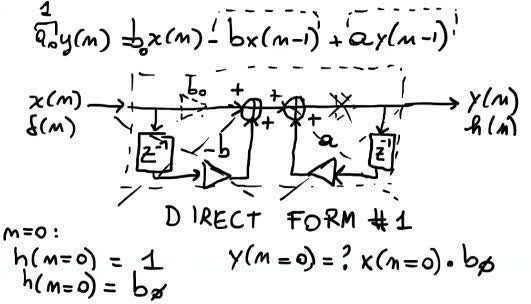
\includegraphics[width=0.8\textwidth]{images/Screenshot from 2022-10-07 16-24-14.png}
\end{center}
Direct form \#1, in this case for $n<0$ the system for us it does not exist, so zero: so $h(n=0)=b_0=1$ in our case

\subsubsection{From generic output to transfer function and complex conjugates}
Consider
$$
y(n)=0.5x(n)-2x(n-1)+x(n-2)-2\rho\cos(\theta)y(n-1)-\rho^2y(n-2)
$$
We can easily find $H(z)$, the coefficients of the $y$ on the right must change sign as they go to the left:
$$
H(z)=\frac{
    0.5-2z^{-1}+z^{-2}
}{
    1+2\rho\cos(\theta)z^{-1}+\rho^2z^{-2}
}
$$
Also $h(n=0)=b_0=0.5$ and $y(n=0)=x(n=0)\cdot 0.5$

The $1+2\rho\cos(\theta)z^{-1}+\rho^2z^{-2}$ represents 2 complex conjugates:
$$
1-2\rho\cos(\theta)z^{-1}+\rho^2z^{-2}\rightarrow \rho(\cos(\theta)\pm j\sin(\theta))
$$
$
1+2\rho\cos(\theta)z^{-1}+\rho^2z^{-2}\rightarrow -\rho e^{\pm j\theta}
\\
1-2\rho\cos(\theta)z^{-1}+\rho^2z^{-2}\rightarrow \rho e^{\pm j\theta}
$

Their product is a real coefficient!

\textbf{In general if the numerator and the denominator are expressed with $z^{-1}$, solve them normally (imposign $z^{-1}=w$ and then invert the results) or exploiting the above formulas then introduce a number of zeros (if solved the denominator) or poles (if solved the numerator) equal to the maximum grade of the polynomial, which will simplify}.

\subsubsection{Maximum phase to minimum phase}
$$
H(z)=h_0+h_1z^{-1}+\cdots+h_Nz^{-N}\Leftrightarrow G(z)=z^{-N}H^*(z^{-1})
$$
The $G$ version will have the same coefficients but in reverse order and \textbf{exact same magnitude}

The roots that are maximum phase will become minimum phase by choosing their reciprocal in conjugate position, an example:
$$
H_M(z)=\frac{
    \left(
        1-2\sqrt{2}z^{-1}+4z^{-2}
    \right)
    \left(
        1+2\sqrt{2}z^{-1}+4z^{-2}
    \right)
}{4+z^{-2}}
$$
The numerator (only it) introduce maximum phase, write their $G$ version:
$$
H_m(z)=\frac{
    \left(
        4-2\sqrt{2}z^{-1}+z^{-2}
    \right)
    \left(
        4+2\sqrt{2}z^{-1}+z^{-2}
    \right)
}{4+z^{-2}}
$$
Alternatively
As $\rho=2$, now $\rho=\frac{1}{2}$:
$$
H_m(z)=A\frac{
    \left(
        1-\frac{\sqrt{2}}{2}z^{-1}+\frac{1}{4}z^{-2}
    \right)
    \left(
        1+\frac{\sqrt{2}}{2}z^{-1}+\frac{1}{4}z^{-2}
    \right)
}{4+z^{-2}}
$$

\subsection{All-pass filter}
It has this form:
$$
H(z)=\frac{c+z^{-1}}{1+cz^{-1}}
$$
\textbf{Has magnitude constant=1, keeps magnitude and changes the phase}. To achieve it place the pole in a reciprocal conjugate position w.r.t. zero (if zero in 2, put pole in $\frac{1}{2}$)
$$
y(n)=cx(n)+x(n-1)-cy(n-1)
$$
More in general it has this form:
$$
H(z)=\frac{
    a_0+a_1z^{-1}+\cdots+a_{n-1}z^{n-1}+a_nz^{-n}
}{
    a_n+a_{n-1}z^{-1}+\cdots+a_1z^{n-1}+a_0z^n
}
$$
    % !TeX root = ../main.tex

\section{Discret Time Fourier Transform (DTFT)}
Discrete time sequence \textbf{non periodic} and I compute a continuous frequency signal (continuous in frequency domain). Defined as
\begin{LARGE}
    $$
    X(f)=\sum_{n=-\infty}^\infty x(n)e^{-j2\pi fn}
    $$
\end{LARGE}
\begin{itemize}
    \item $f$ is the normalized frequency in $[0,1)$ or $[-0.5,0.5)$
    \item $\omega=2\pi f$ is the normalized angular frequency in $[0,2\pi)$ or $[-\pi,\pi)$
    \item DTFT is periodic with period = 1 in normalized frequency, period = $2\pi$ in normalized omega, period = $Fs$ in frequency [Hz]
\end{itemize}

\subsection{Properties}
\begin{itemize}
    \item DTFT$\brackets{x(n)*y(n)}=X(f)\cdot Y(f)$
    \item DTFT$\brackets{x(n-k)}=X(f)\cdot e^{-j2\pi fk}$
    \item If $x(n)$ is real, $X(f)=X^*(-f)$, symmetric behavior
    \item Relationship with Z-transform: $X(f)=X(z)\Big|_{|z|=1}$
\end{itemize}
Given
$$
H(z)=\frac{
    \sum_{k=0}^Nb_kz^{-k}
}{
    \sum_{k=0}^Da_kz^{-k}
}\Rightarrow H(f)=H(z)\Big|_{|z|=1}
$$
\begin{itemize}
    \item The amplitude is
    $$
    |H(f)|=|H(z)|\Big|_{|z|=1}=\frac{
        \left|\sum_{k=0}^Nb_kz^{-k}\right|
    }{
        \left|\sum_{k=0}^Da_kz^{-k}\right|
    }\Bigg|_{|z|=1}
    $$
    \item The phase (depends on the zeros, not on the poles) is
    $$
    \angle(H(f))=\angle(H(z))\Big|_{|z|=1}=\angle\left(
        \sum_{k=0}^Nb_kz^{-k}
    \right)-\angle\left(
        \sum_{k=0}^Da_kz^{-k}
    \right)\Bigg|_{|z|=1}
    $$
\end{itemize}
    % !TeX root = ../main.tex

\section{Discret Fourier Transform (DFT)}
Discrete time sequence \textbf{periodic}. Discrete both in time and frequency, finite number/summation:
\begin{LARGE}
    $$
    X(k)=\sum_{n=0}^{N-1} x(n)e^{-j2\pi \frac{k}{N}n}
    $$
\end{LARGE}
$X(k)$ with $k=[0,N-1]$. While DTFT is continuous in the frequency domain
$$
X(f)=\sum_{n=-\infty}^\infty x(n)e^{-j2\pi fn}
$$
\textbf{In the DFT we assume that the period is signal w.r.t. provided N}

\subsection{Relationship with DTFT}
\begin{itemize}
    \item While in DTFT $f\in\,\,[0,1)$, with DFT $f=\left[0,\frac{1}{N},\cdots,\frac{N-1}{N}\right]\rightarrow$ length of $N$
    \item The inverse (IDFT):
    $$
    x(n)=\frac{1}{N}\sum_{k=0}^{N-1}X(k)e^{2j\pi\frac{k}{N}n}
    $$
    Length of $N$
    \item \textbf{DFT==DTFT only if FIR}, if IIR we are truncating when applying DFT, losing info
    \item DTFT continuous over frequencies, DFT discrete
    \begin{itemize}
        \item Sampling in Fourier = periodicity in time
        \item Sampling in time = periodicity in frequency/Fourier
    \end{itemize}
    \item Both DFT and IDFT are periodic with a period of $N$ samples:
    $$
    X(k+tN)=X(k)\qquad\forall\,\,t\in[-\infty,\infty]
    $$
    $$
    x(n)=IDFT(X(k))=x(n+tN)\qquad\forall\,\,t\in[-\infty,\infty]
    $$
\end{itemize}

\subsection{DFT as a matrix product}
The DFT of a sequence $x(n)$ can be computed by:
$$X=W_N\cdot x$$
Where:
$$
W_N=
\begin{bmatrix}
    W_i^0 & W_i^0 & W_i^0 & W_i^0 & \cdots & W_i^0\\
    W_i^0 & W_i^1 & W_i^2 & W_i^3 & \cdots & W_i^{N-1}\\
    W_i^0 & W_i^2 & W_i^4 & W_i^6 & \cdots & W_i^{2(N-1)}\\
    W_i^0 & W_i^3 & W_i^6 & W_i^9 & \cdots & W_i^{3(N-1)}\\
    \vdots & \vdots & \vdots & \vdots & \ddots & \vdots\\
    W_i^0 & W_i^{N-1} & W_i^{2(N-1)} & W_i^{3(N-1)} & \cdots & W_i^{(N-1)^2}        
\end{bmatrix}=
$$
$$
=
\begin{bmatrix}
    1 & 1 & 1 & 1 & 1\\
    1 & e^{-j2\pi/N} & e^{-j4\pi/N} & \cdots & e^{-j2\pi(N-1)/N}\\
    1 & e^{-j4\pi/N} & e^{-j8\pi/N} & \cdots & e^{-j4\pi(N-1)/N}\\
    1 & \cdots & \cdots & \cdots & \cdots\\
    1 & e^{-j2\pi(N-1)/N} & e^{-j4\pi(N-1)/N} & \cdots & e^{-j2\pi(N-1)(N-1)/N}
\end{bmatrix}
$$
\begin{LARGE}
    $$W_i=e^{-j\frac{2\pi}{i}}$$
\end{LARGE}
Or
$$
W_N=e^{-j\frac{2\pi}{N}kn}
$$
$$
\underline{k}=\left[0,1,\cdots,N-1\right]
$$
$$
\underline{n}=\left[0,1,\cdots,N-1\right]
$$
\textbf{The inverse of $W:\,\,N\times N$ is its conjugate transpose divided by $N$}.
$$y(n)=W^{-1}Y(k)$$

\textbf{If using matrices, $Y(k)=X(k)\cdot H(k)$ element-wise product}.

\subsection{Zero padding}
Zero padding means windowing, which will result in a sinc behavior in the Fourier domain. When we compute the DFT, if the repetition of the signal results in discountinuities:
\begin{center}
    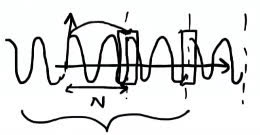
\includegraphics[width=0.5\textwidth]{images/zero_pad_01.png}
\end{center}
We introduce zero till we get a signal that repeated will not have discountinuities. This new signal obtained is made of the product of two signals: itself and a rectangle that ends where the previous signal ended (will become 0 onward, so $N_{pad}$ must be multiple of period)
\begin{center}
    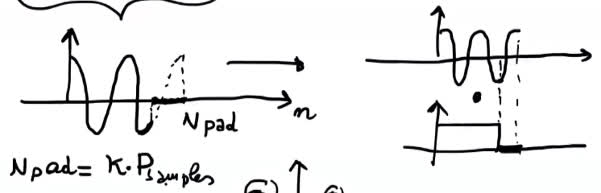
\includegraphics[width=0.8\textwidth]{images/zero_pad_02.png}
\end{center}
In the Fourier/frequency domain so we will get the \textbf{convolution} of transform of those two signals: the transform of the first will be two pulses ($\delta$) at the peaks, while the transform of the rectangle will be a sinc.\\
Convolving the two, we will get two sincs due to the effect of the window, each one the peaks (in the example peaks at $2Hz$ as frequency of sinusoid $f_0=2Hz$):
\begin{center}
    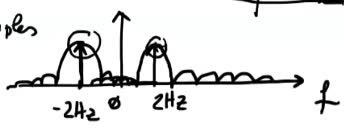
\includegraphics[width=0.5\textwidth]{images/zero_pad_03.png}
\end{center}
But when discretize the DFT, we should be careful to put the peak $x$ in the axis/in the interval plotted:
$$k\frac{F_s}{N_{pad}}=f_0$$
$$N_{pad}=k\frac{F_s}{f_0}=k\cdot P_{samples}$$
Same conclusion as before.

But if \textbf{strong density} in the spectrum (a lot of padded zeros), introducing a sinc and the peak will not be exactly at $f_0$, small overlap on the maximum
due to tails, introduced errors.

\subsubsection{Conditions}
\begin{enumerate}
    \item $N_{pad}=k\cdot P_{samples}$. \textbf{If 2+ signals summed, the global period in samples is the least common multiple (mcm) of the periods}. What if one of the periods is not an integer?
    $$
    \begin{cases}
        P_1=25\\
        P_2=\frac{50}{2.2}=\frac{250}{11}
    \end{cases}
    $$
    $$
    lcm(25,\frac{250}{11})=lcm(25,250)=250
    $$
\end{enumerate}

\subsubsection{Alternative to zero-padding for discountinuities in DFT}
When we are windowing we have a rectangular behavior. If its length is $N$, its first zero is $\frac{1}{N}$
\begin{center}
    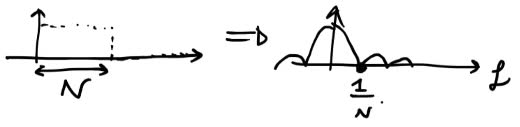
\includegraphics[width=0.7\textwidth]{images/zero_pad_04.png}
\end{center}
Suppose a signal with 50 samples, the size of the main lobe we are introducing in the frequency (the first zero) is $\frac{1}{50}$ in the normalized domain or $\frac{1}{50}F_s$ in the $Hz$ domain. Suppose $F_s=50$:
\begin{center}
    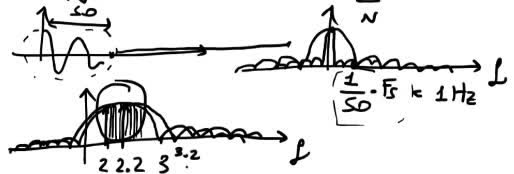
\includegraphics[width=0.7\textwidth]{images/zero_pad_05.png}
\end{center}
Two lobes sum up, so using zero-padding useless. We have to reduce size of main lobe of the sinc: increasing number of samples.
\begin{center}
    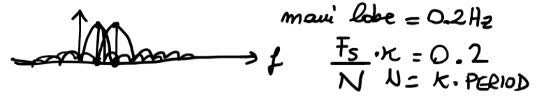
\includegraphics[width=0.7\textwidth]{images/zero_pad_06.png}
\end{center}
So the Alternative is to redefine the signals in time domain with samples equal to the global period in samples immediately: \textbf{more measurement, add more samples}.

\subsection{Discontinuity}
In the Fourier domain introduces high frequency content

\subsection{DFT of sinusoids: pulses and peaks}
A sinusoid (a cosine) with frequency $f_0$ will have two $\delta$'s in the frequency domain, one at $f_0$ the other at $-f_0=F_s-f_0$ (mirrored w.r.t. $F_s/2$ Nyquist, if normalized frequencies, it is at $1-\tilde{f}_0$, $\pm\tilde{\omega}_0$). If we add a second signal with a different frequency $f_0'$, we will have two additions $\delta$'s at $f_0'$ and $-f_0'$. In the magnitude/amplitude plot, the two pulses will have $\frac{N}{2}$ height

Given a sinusoid with $F_s$ [Hz] and $f_0$ [Hz], its DFT will have two peaks, one in $f_0$, the other one in $F_s-f_0$, symmetric w.r.t. the Nyquist frequency. For example, given:
$$
x(t) = A*\cos(2\pi f_0t)\qquad F_s = 50Hz\qquad f_0 = 2Hz
$$
$$
x(n) = A*\cos\left(\frac{2\pi}{25}n\right)
$$
Its DFT is:
$$
|X(\omega)|=\frac{N}{2}\delta\left(\omega-\frac{2\pi}{25}\right)+
\frac{N}{2}\delta\left(\omega-\left(2\pi-\frac{2\pi}{25}\right)\right)
$$

\subsection{DFT and IDFT periodicty}
Given a non periodic sequence $x(n)$ defined over $N$ samples, its $N$-periodic extension is defined as:
$$
\tilde{x}(n)=\sum_{t=-\infty}^\infty x(n-tN)
$$
Same with DFT:
$$
\tilde{X}(k)=\sum_{t=-\infty}^\infty X(k-tN)
$$

\subsubsection{Cyclic/circular convolution}
For the DFT:
$$
X_1(k)\cdot X_2(k) \neq x_1(n)* x_2(n)
$$
$$
IDFT\Brackets{X_1(k)\cdot X_2(k)}= x_1(n)\circledast x_2(n)=\sum_{m=0}^{N-1}x(m)\tilde{y}(n-m)
$$
The cyclic/circular convolution holds
\begin{center}
    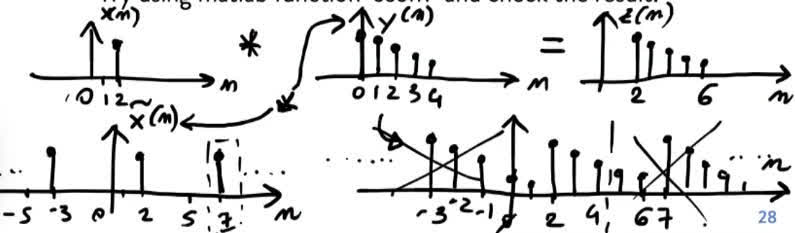
\includegraphics[width=1\textwidth]{images/cyclic_conv.png}
\end{center}
\textbf{So to compute circular convolution I can use the DFT: compute product of DFTs and then invert}.

\textbf{But LTI systems such as communication, radar, audio and image systems all work with linear convolution, so to compute linear convolution in DFT how do we do?}

\subsubsection{Linear and cyclic convolution}
Given a sequence with length $L$ and a sequence with length $P$, the maximum length of the linear convolution is $N_c=L+P-1$.
\begin{center}
    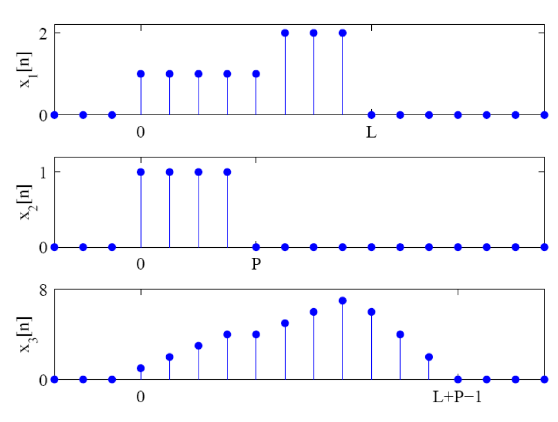
\includegraphics[width=1\textwidth]{images/cyclic_conv_01.png}
\end{center}
The cyclic convolution computed over a generic number $N$ of samples is equal to the linear convolution if $N$ is long enough to avoid periodic artifacts. Therefore
$$
N\geq L+P-1
$$
\textbf{Pad with zeros the two sequences until reaching $N$ samples, we will not introduce artifacts and the result of the cyclic convolution will be equal to that of the normal convolution}.

\subsection{Long convolution}
The input sequence $x(n)$ can be very long, zero-padding can be unfeasible if it is unknown as well (real-time applications), so we can segment the signal into smaller blocks and process them separately

\subsubsection{Overlap and add}
\begin{itemize}
    \item Let the impulse resposne $h(n)$ long $P$, decompose the input $x(n)$ into \textbf{non-overlapped} blocks with length $L$
    \item For each block compute the output as
    $$IDFT(X_n(k)\cdot H(k)),k\in [0,N=L+P-1)$$
    \item Sum the overlapping portions between the results
\end{itemize}

\subsubsection{Overlap and save}
\begin{itemize}
    \item Let the impulse resposne $h(n)$ long $P$, decompose the input $x(n)$ into \textbf{overlapped} blocks with length $L>P$ with overlap $P-1$
    \item The circular convolution evaluated over $L$ sampels is different from the linear convolution only in the first $P-1$ samples (periodic artifacts)
    \item Pad the first block with $P-1$ zeros at the beginning
    \item Overlap blocks by $P-1$ samples
    \item For each block compute the circualr convolution ofer $L$ samples and discard the first $P-1$ samples
    $$IDFT(X_n(k)\cdot H(k)),k\in [0,N=L+P-1)$$
    \item Sum the overlapping portions between the results
\end{itemize}
    % !TeX root = ../main.tex

\section{1D Digital filters}
\begin{center}
    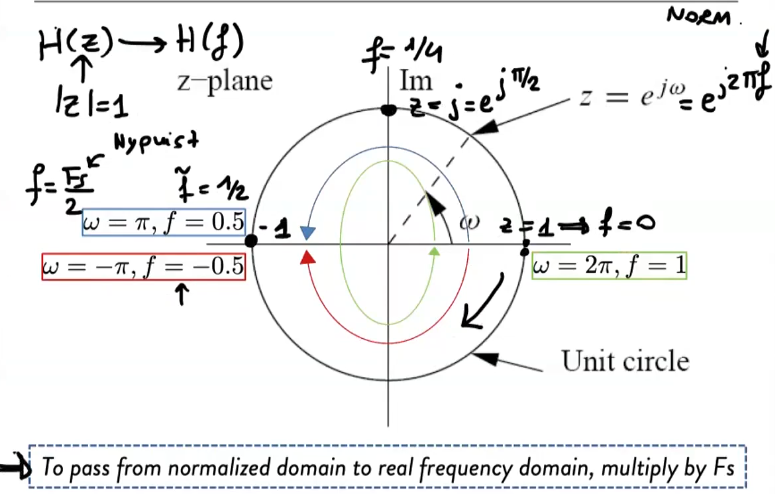
\includegraphics[width=1\textwidth]{images/zero_pole.png}
\end{center}
If asks for $Hz$ domain, multiply by $F_s$. Reminder, a filter:
\begin{LARGE}    
    $$
    H(z)=\frac{
        \sum_{k=0}^Nb_kz^{-k}
    }{\sum_{k=0}^Da_kz^{-k}}=
    z^{D-N}\frac{b_0}{a_0}\frac{
        \prod_{i=1}^N(z-z_i)
    }{\prod_{i=1}^N(z-p_i)}=
    \frac{b_0}{a_0}\frac{
        \prod_{i=1}^N(1-z_iz^{-1})
    }{\prod_{i=1}^N(1-p_iz^{-1})}
    $$
\end{LARGE}
\begin{itemize}
    \item The poles
    \begin{itemize}
        \item Are associated with the autoregressive part, they generate IIR filter $z\rightarrow p_i$, in the frequency the filter will increase $H(f)$
        \item The filter amplitude response enhances frequencies which are near the poles
        \item If poles are outside the unit circle and the filter is causal, the system is unstable
    \end{itemize}
    \item The zeros
    \begin{itemize}
        \item Are associated with the moving average of the filter, they generate FIR filters
        \item The filter amplitude response attenuates frequencies which are near the zero
        \item Zeros influence also the phase of the filter (they do not influence stability)
        \begin{itemize}
            \item Minimum phase zeros if $z<1$, inside unit circle
            \item Maximum phase zeros if $z\geq 1$, outside unit circle
        \end{itemize}
    \end{itemize}
\end{itemize}

\subsection{Filter design: remarkable LTI filters}
\begin{itemize}
    \item Place poles close tot he unit circle in frequencies that must be emphasized
    \item Place zeros according to the desired phase response, the closer are to the unit circle the higher frequency attenuation
\end{itemize}

\subsubsection{Notch}
I want to delete a specific frequency:
\begin{enumerate}
    \item Put two complex zeros on the unit circle
    \item Put two poles with absolute value less than 1, close to unit circle
\end{enumerate}
\begin{center}
    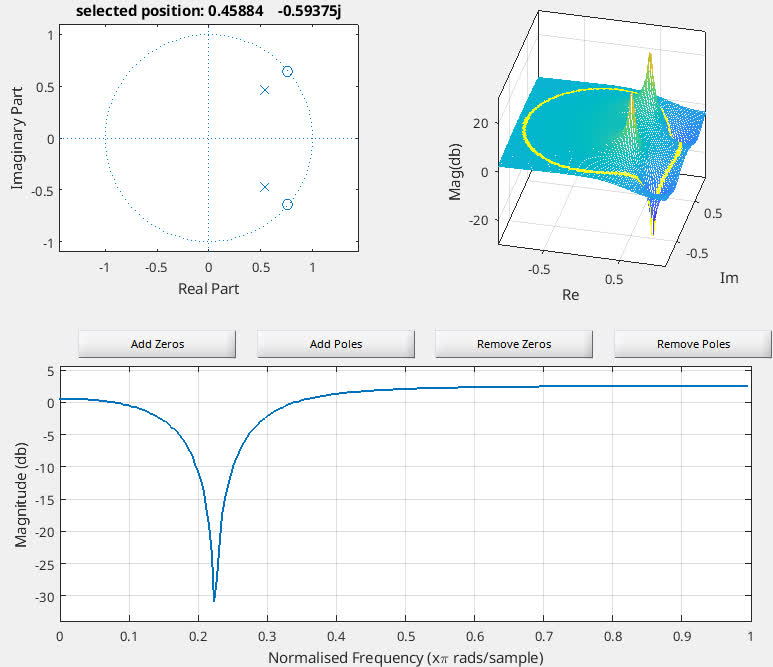
\includegraphics[width=1\textwidth]{images/notch.png}
\end{center}

\subsubsection{Magnitude square function}
The magnitude response of a LTI system is:
$$
M(f)=|H(f)|^2=H(f)\cdot H^*(f)=H(z)\cdot H^*(z^{-1})\big|_{|z|=1}
$$
Given a generic rational transfer function
$$
H(z)=\frac{b_0}{a_0}\frac{
    \prod_{i=1}^N(1-z_iz^{-1})
}{\prod_{i=1}^N(1-p_iz^{-1})}
$$
$$
\Downarrow
$$
$$
M(z)=H(z)H^*(z^{-1})=\frac{|b_0|^2}{|a_0|^2}
\frac{
    \prod_{i=1}^N(1-z_iz^{-1})(1-z_i^*z)
}{\prod_{i=1}^D(1-p_iz^{-1})(1-p_i^*z)}
$$
Where $H^*(z^{-1})$ means $H(z)$ with complex conjugates evaluated in $z^{-1}$, star in the coefficients
\begin{itemize}
    \item For each zero $z_i$ of $H(z)$ there is another zero at $\frac{1}{z_i^*}$
    $$
    \frac{1}{z_i^*}=\frac{1}{\rho_ie^{-j\theta_i}}=\frac{1}{\rho_i}e^{j\theta_i}
    $$
    The angle/phase is the same, only distance from origin changes
    \item For each pole $p_i$ of $H(z)$ there is another pole at $\frac{1}{p_i^*}$
    \item $M(z)$ presents poles and zeros in conjugate reciprocal pairs
\end{itemize}
\begin{center}
    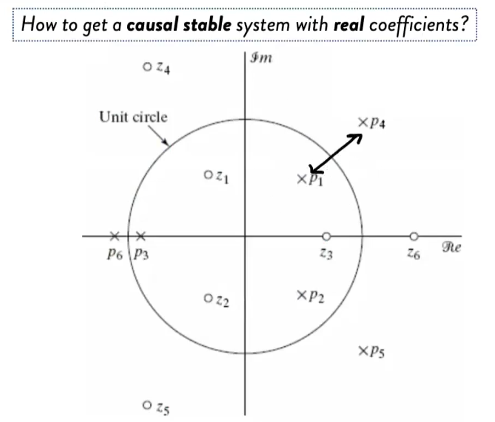
\includegraphics[width=0.6\textwidth]{images/magnitued_square.png}
\end{center}
Given a magnitude response requirement $M(z)$ for $H(z)$, given stability and causality requirements for $H(z)$:
\begin{itemize}
    \item The poles of $H(z)$ are those of $M(z)$ inside the unit circle anda re uniquely identified (for stability constraints)
    \item The zeros of $H(z)$ are not uniquely identified (as zeros influence only the phase and we have no constraints on phase), so the zeros can be both inside and outside the unit circle
    \item Given a causal FIR filter $H(z)$ of order $N$, it has the same magnitude  response $M(z)$ of the causal FIR filter:
    $$G(z)=z^{-N}H^*(z^{-1})$$
    Minimum to maximum phase filter and viceversa
\end{itemize}
From the previous example, in order to have causal and stable system we select the following zeros and poles:
\begin{center}
    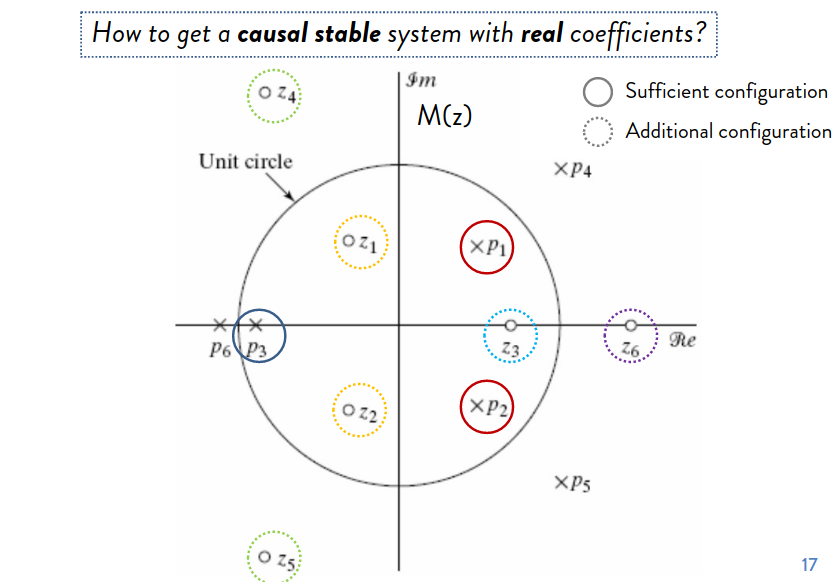
\includegraphics[width=0.6\textwidth]{images/magnitued_square2.png}
\end{center}

\subsubsection{Allpass filters}
Flat behavior in the frequency, which means constant gain and any phase:
$$
|H_{ap}(f)|=|H_{ap}(z)|\big|_{|z|=1}=1\qquad\forall f
$$
Given the previous considerations, a generic causal allpass filter is:
$$
H_{ap}(z)=z^{-K}e^{j\phi}\frac{A(z)}{\tilde{A}(z)}
$$
Where
$$
\begin{cases}
    A(z)=1+a_1z^{-1}+a_2z^{-2}+\cdots+a_Nz^{-N}\\
    \tilde{A}(z)=z^{-N}A^*(z^{-1})=a^*_N+a_{N-1}^*z^{-1}+\cdots+a_2^*z^{2-N}+a_1^*z^{1-N}+z^{-N}
\end{cases}
$$
The denominator is the G version of the numerator, so their magnitudes cancel out.
$$
H_{ap}(z)=z^{-N}e^{j\theta}
\frac{
    1+a_1z^{-1}+a_2z^{-2}+\cdots+a_Nz^{-N}
}{
    a^*_N+a_{N-1}^*z^{-1}+\cdots+a_2^*z^{2-N}+a_1^*z^{1-N}+z^{-N}
}
$$
A general form to represent an allpass real valued impulse response is:
\begin{center}
    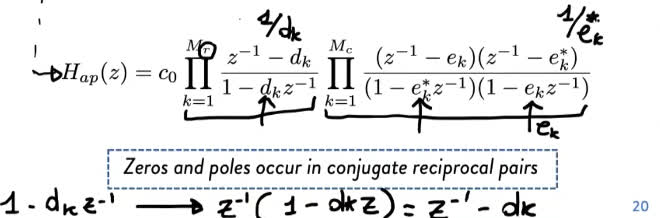
\includegraphics[width=0.6\textwidth]{images/allpass.png}
\end{center}
We introduced a coefficient $c_0$ in order to guarantee magnitude of 1. Basically
$$
H(z)=\left|c_0\frac{B_{ap}(z)}{A_{ap}(z)}\right|_{|z|=1}=1
$$
We pass to the frequency domain. As that fraction is flat in the frequency domain, we choose frequency $f=0,z=1$:
$$
|c_0|\frac{|B_{ap}(z=1)|}{|A_{ap}(z=1)|}=1
$$
$$
\Rightarrow c_0 = \pm\frac{|A_{ap}(z=1)|}{|B_{ap}(z=1)|}
$$
So to find $c_0$ just sum  all the coefficients and then compute the division.

\textbf{Zeros and poles are in conjugate reciprocal pairs}.
Properties:
\begin{itemize}
    \item Cascade of two allpass filters is again an allpass filter
    \item Each pole of an allpass system is associated with a conjugate reciprocal zero
    \item The magnitude of many cascaded allpass filters is always the same
\end{itemize}

\subsubsection{Minimum phase filters}
\begin{itemize}
    \item Minimum phase filters are such that both $H(z)$ and $\frac{1}{H(z)}$ are stable and causal
    \item The poles must be inside the unit circle
    \item The zeros must be inside the unit circle
    \item Given a square magnitude response $M(z)$, there is a unique system whose zeros and poles are inside the unit circle and it is called minimum phase system
\end{itemize}
\begin{center}
    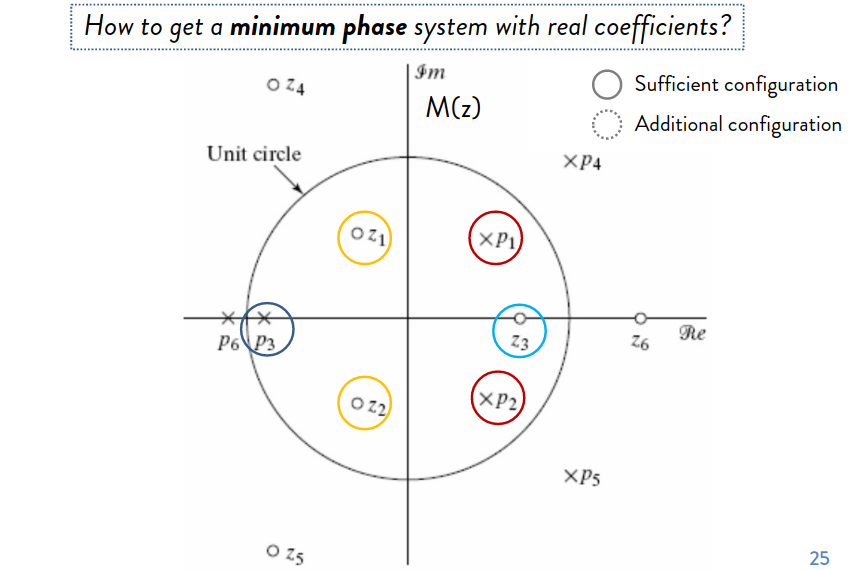
\includegraphics[width=0.8\textwidth]{images/minphase.png}
\end{center}
Properties of allpass: \textbf{Any rational causal stable system can be decomposed into the multiplication of a minimum phase system and an allpass system}
$$
H(z)=H_{min}(z)H_{ap}(z)
$$
Causal and stable, so all poles are inside the unit circle!\\
$H_{min}(z)$ contains:
\begin{itemize}
    \item The poles and the zeros of $H(z)$ that lie inside the unit circle
    \item Zeros that are conjugate reciprocals of the zeros $H(z)$ lying outside the unit circle
\end{itemize}
$H_{ap}(z)$ contains:
\begin{itemize}
    \item All the zeros of $H(z)$ that lie outside the unit circle
    \item Poles that are conjugate reciprocals of the zeros of $H(z)$ lying outside the unit circle
\end{itemize}

\subsection{Digital filters' design}
\begin{enumerate}
    \item Specify always the characteristics of the filter in frequency domain, not in time domain (e.g. lowpass, highpass, bandpass...)
    \item Approximate these properties using a discrete-time system, find the filter coefficients
    \item Realize the system using finite precision arithmetic
\end{enumerate}

\subsubsection{Ideal filters}
\begin{center}
    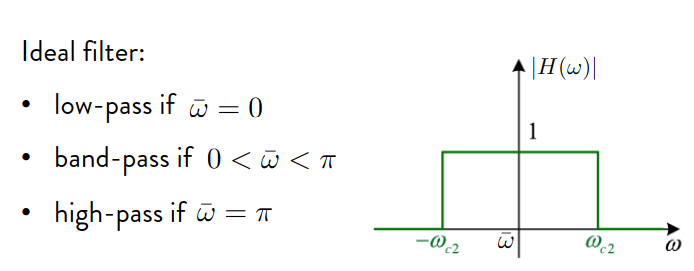
\includegraphics[width=0.8\textwidth]{images/idealfilter.png}
\end{center}
Outside the rectangle is called \textbf{stopband}. The impulse response of this filter is $\approx$ the sinc function. It is \textbf{non-causal (sinc has on the left non-causal part)} with an \textbf{infinite delay}, \textbf{real systems can only approximate}.

\subsubsection{Real filters}
\begin{center}
    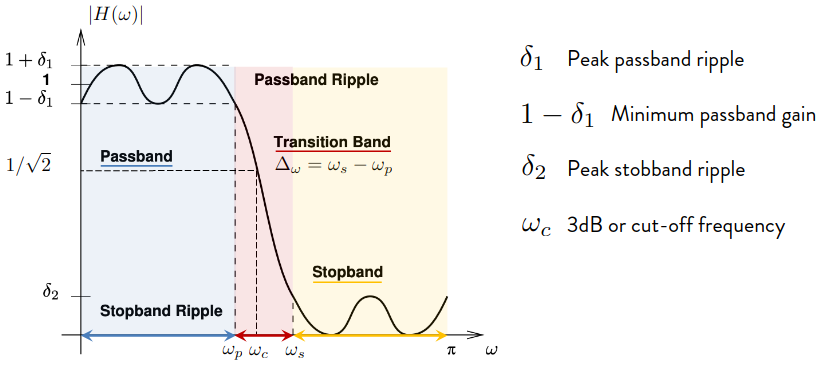
\includegraphics[width=1\textwidth]{images/realfilter.png}
\end{center}
Oscillations both in passband and in stopband. Cutoff frequency is the frequency in which I pass from the passband to the stopband.

As I don't want ripples and we want transition band to 0:
\begin{itemize}
    \item Peak ripple $\rightarrow$ 0
    \item Transition band $\rightarrow$ 0
\end{itemize}
We consider FIR and IIR cases:
\begin{center}
    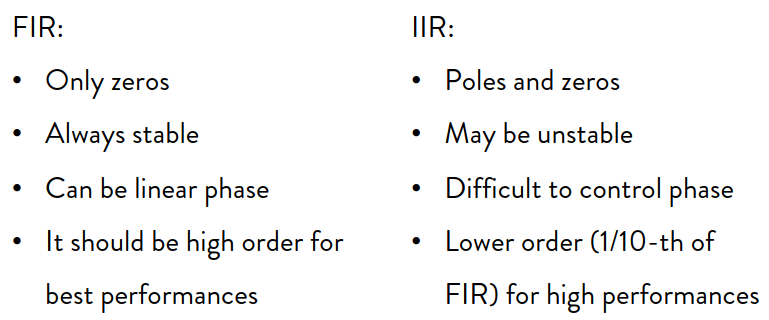
\includegraphics[width=1\textwidth]{images/IIRvsFIR.png}
\end{center}
Allpass must be FIR.

\subsubsection{FIR filter design: windowing method}
I want a rectangle in the frequency, but in the time I have a sinc: obtain a FIR filter by truncating an infinite duration impulse response
\begin{itemize}
    \item Given the ideal $h_i(n)$, build $h(n)=h_i(n)w(n)$
    \item $w(n)$ is a finite duration window, in frequency domain it becomes convolution
    \item $H(f)$ is a blurred version of the ideal filter $H_i(f)$
\end{itemize}
\textbf{Windowing means multiplying in the time, so in the frequency we have convolution}.

How to choose the window? Tradeoff
\begin{itemize}
    \item As short as possible (in time) to minimize the cost of the FIR filter
    \item As narrow as possible in frequency to approach the ideal filter (a narrow in the time means very large in the frequency domain)
\end{itemize}
I want a short signal in the time, so an impulse, $W(f)$ should look like a $\delta(f)$, without considering the filter cost
\begin{itemize}
    \item Its energy must be concentrated around $f=0$
    \item $W(f)$ should decay fast as frequency increases
\end{itemize}
\begin{center}
    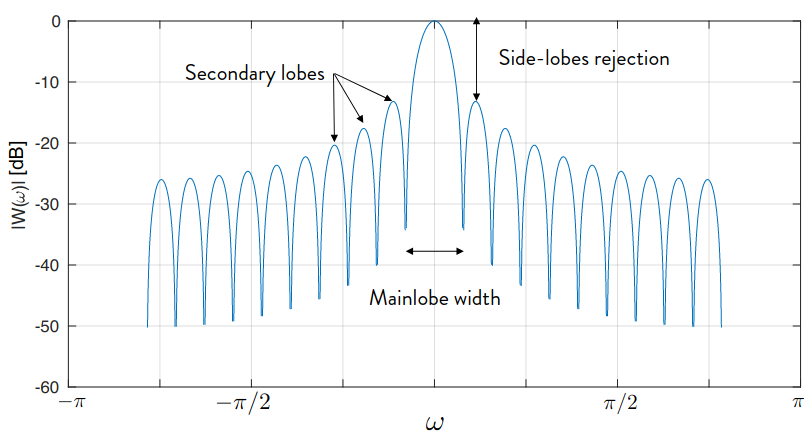
\includegraphics[width=1\textwidth]{images/lobe.png}
\end{center}
We want a big ration of $\frac{width(MainLobe)}{width(SecondaryLobes)}$. Every window is characterized by:
\begin{itemize}
    \item Main-lobe width: it decreases as the window length increases
    \item Side-lobes rejection: ratio between the main-lobe peak and 1° secondary lobe peak [dB], if I want it high for example the blackman window is quite good
    \item Side-lobes roll off: asymptotic decay of the side-lobe peaks vs frequency octave [dB/octave] or frequency decade [dB/decade]
\end{itemize}
\textbf{In matlab set cutoff = double of desired one, if I want cutoff of 0.5 I will put in matlab 1}.

\textbf{Filter order is always \#filter samples-1, e.g. if filter samples = 64, filter order = 64-1 = 63}.

\subsection{Aspects to remember}
\begin{itemize}
    \item \textbf{Phase is always correlated with a delay in the time}
    \item \textbf{Real filters always introduce a delay, a phase term, hence LPF's introduce delays}
    \item \textbf{FIR are always stable}, the numerator has greater grade than denominator
    \item \textbf{Only poles at the origin means FIR}
    \item \textbf{Denominator = 1 means FIR}
    \item \textbf{Maximum phase} will result in \textbf{jumps in the phase plot, specifically jumps of $2\pi$}
    \item \textbf{Minimum phase has the greatest part of energy of the filter concentrated in the first part of the temporal samples}, which means I am introducing very small delay
    \item \textbf{Allpass MUST be FIR}
    \item \textbf{A causal stable allpass system has always maximum phase
    zeros}, they are the reciprocal complex conjugate of the poles therefore the \textbf{phase has jumps = $2\pi$}
    \item \textbf{DFT of sinusoid will have peak in the freq/normalized freq depending on representation of frequency domain (either $f_0\,\,[Hz]$ or $\tilde{f_0}$) and another one symmetric w.r.t. Nyquist frequency, and in presence of consine with magnitude $A$, in DFT domain we will have a pulse of magnitude $A/2$}
    \item \textbf{To attenuate a sinusoid signal of $\tilde{\omega}$, and to have real coefficients in $H$, put zeros in $Ae^{j\tilde{\omega}}$, and in $Ae^{-j\tilde{\omega}}$, $b=poly([zeros])$, to enhance put poles instead with the same criteria. OTHER SIGNALS WILL BE INFLUENCED AS WELL.}
    \item \textbf{To delete (attenuate) a signal with a frequency $\tilde{\omega}$ WITHOUT INFLUENCING OTHERS SIGNALS we construct a notch: put 2 conjugate zeros in $1\cdot e^{j\tilde{\omega}}$ and 2 conjugate poles in $\rho\cdot e^{j\tilde{\omega}}$, with $\rho<1$} 
\end{itemize}
    % !TeX root = ../main.tex

\section{Multirate Processing}
\subsection{Downsampling}
    \begin{LARGE}
        $$
        y(n)=x(nM)
        $$
    \end{LARGE}
    \begin{center}
        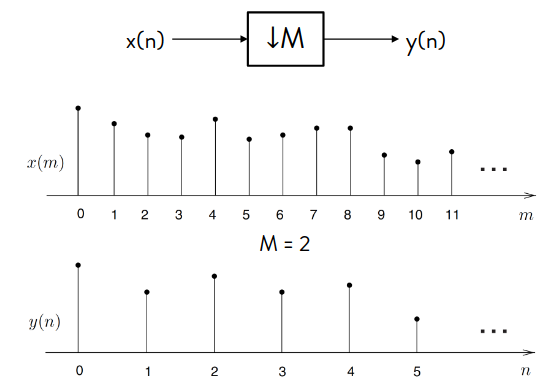
\includegraphics[width=0.9\textwidth]{images/downsampling.png}
    \end{center}
    In the frequency domain, the downsampled is:
    $$
    Y(f)=\frac{1}{M}\sum_{k=0}^{M-1}X\left(\frac{f-k}{M}\right)
    $$
    The DTFT if $y(n)$ is composed of copies of the DTFT of $x(n)$ \textbf{expanded by M and repeated with period 1} in normalized frequency (or $F_s$ in Hertz, or $2\pi$ in angular frequencies)

    \textbf{The gain is reduced by a factor of M}.
    
    \textbf{In practice the DFT of a downsampled sinusoid will be the pulses evaluated at $\tilde{\omega}\cdot M$ with a gain reduced by $M$: $A\rightarrow \frac{A}{M}$, remember to add the symmetric pulse for each!}

    \subsubsection{Aliasing}
    \begin{center}
        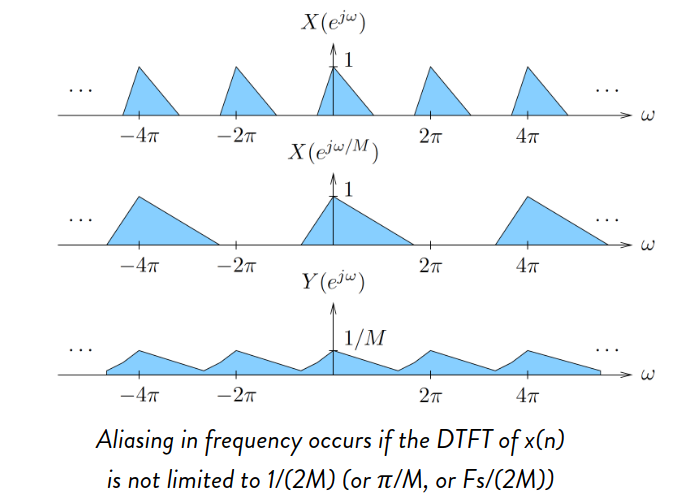
\includegraphics[width=0.9\textwidth]{images/downsampling_aliasing.png}
    \end{center}
    \textbf{Note that in the picture it is not a real signal, not symmetric}.

    There isn't overlap if
    $$
    BM\leq \frac{1}{2}\leftrightarrow B\leq\frac{1}{2M}\leftrightarrow B\leq\frac{\pi}{M}\leftrightarrow B\leq\frac{F_s}{2M}
    $$
    Where $B$ is the first right zero in frequency diagram, the original band of my signal. To avoid aliasing, we introduce a lowpass filter.

    \subsubsection{Decimation}
    Put a lowpass filter, then downsample. We use a lowpass with cutoff of $\frac{1}{2M}$:
    $$
    H(f)=\begin{cases}
        1\qquad |f|\leq\frac{1}{2M}\\
        0\qquad\text{otherwise}
    \end{cases}
    $$
    \begin{center}
        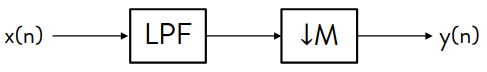
\includegraphics[width=0.5\textwidth]{images/downsampling_lpf.png}
    \end{center}

\subsection{Upsampling}
    Upsampling of a factor L means to insert L -1 zeros between the input signal samples
    \begin{LARGE}
        $$
        y(n)=\begin{Bmatrix}
            x(n/L) & n=kL\\
            0 & \text{otherwise}
        \end{Bmatrix}
        $$    
    \end{LARGE}
    \begin{center}
        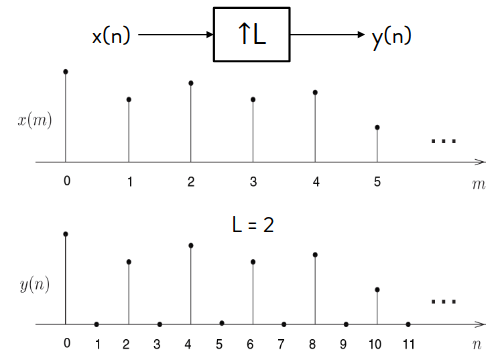
\includegraphics[width=0.9\textwidth]{images/upsampling.png}
    \end{center}
    In the frequency domain:
    $$
    Y(f)=X(fL)
    $$
    Upsampling compresses the DTFT by a factor of $L$, \textbf{if we upsampled a sinusoid, its DFT will repeat the pulses every $L$, same goes for the symmetric pulses}.

    \textbf{In practice the DFT of an upsampled sinusoid will be the pulses evaluated at $\frac{\tilde{\omega}+2\pi k}{L}$, where $k=0,1,\cdots,L-1$, remember to add the symmetric pulse for each!}

    \subsubsection{Replicas}
    \begin{center}
        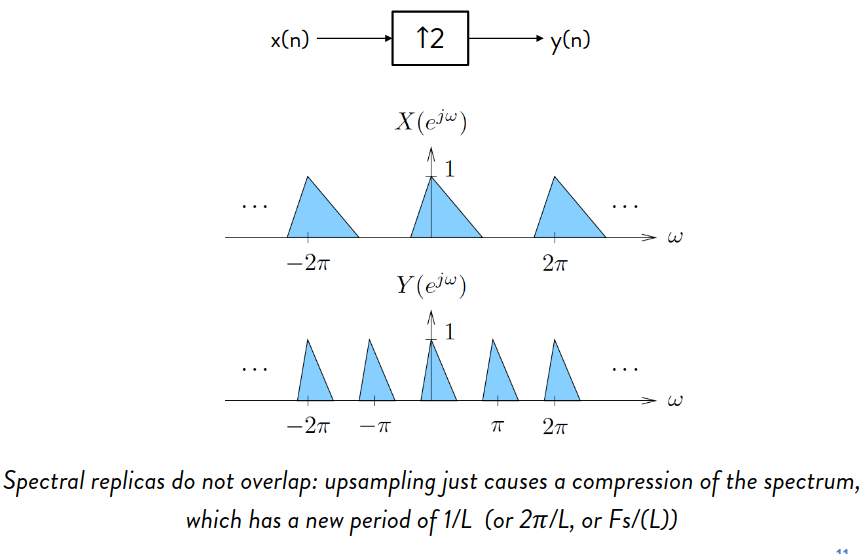
\includegraphics[width=0.9\textwidth]{images/upsampling_replica.png}
    \end{center}

    \subsubsection{Interpolation}
    Put a lowpass filter \textbf{after} upsampling. We use a lowpass with cutoff of $\frac{1}{2L}$, in this way we remove replicas:
    $$
    H(f)=\begin{cases}
        L\qquad|f|\leq\frac{1}{2L}\\
        0\qquad\text{otherwise}
    \end{cases}
    $$
    \begin{center}
        \includegraphics[width=0.5\textwidth]{images/upsampling_Interpolation.png}
    \end{center}
    \textbf{After lpf, MULTIPLY AGAIN THE SIGNAL BY L}

\subsection{Rational sampling rate conversion: noninteger factor}
    Cascade interpolator wih a decimator
    \begin{center}
        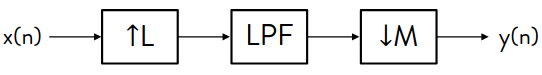
\includegraphics[width=0.5\textwidth]{images/rationalsampling.png}
    \end{center}
    The lowpass dilter is:
    $$
    H(f)=\begin{cases}
        L\qquad|f|\leq\min\Brackets{\frac{1}{2L},\frac{1}{2M}}\\
        0\qquad\text{otherwise}
    \end{cases}
    $$

    % !TeX root = ../main.tex

\section{Matlab}

\begin{lstlisting}[language=Matlab, escapeinside=`']
    close all
    clearvars
    clc
\end{lstlisting}

\subsection{Cosine signals}

    \subsubsection{Sinusoid signal continuous, in time and in samples plot}
    A sinusoid in continuous domain is
    $$
    x(t)=A\cdot\cos(2\pi ft+\phi)
    $$
    Its sampled version is:
    $$
    \begin{cases}
        x(n)=A\cdot\cos(2\pi \tilde{f}n+\phi)\\
        \tilde{f}=\frac{f}{F_s}
    \end{cases}
    $$
    Given:
    $$
    \begin{cases}
        t=[0,0.5]\\
        F_s=1000\,\,Hz=\frac{1}{T_s}\qquad\text{sampling rate}\\
        A=0.8\qquad\text{amplitude}\\
        f=50\,\,Hz\qquad\text{frequency, not normalized}\\
        \phi=30^\circ=\frac{\pi}{6}\qquad\text{phase}
    \end{cases}
    $$
    In matlab:
    \begin{lstlisting}[language=Matlab, escapeinside=`']
        A = 0.8;
        f = 50;
        Fs = 1e3; %1000;
        Ts = 1/Fs;
        t = 0:Ts:0.5;
        phi = 30; % deg
        
        % conversion
        % phi_deg:phi_rad = 180: pi
        phi_rad = phi*pi/180;
        
        x = A*cos(2*pi*f*t + phi_rad);

        %% Plot the signals as a function of time and as a function of samples

        figure(1);
        plot(t, x);
        hold on;
        plot(t, x1, '--');
        title('Signals as a function of time');

        figure(2);
        plot(x); %plot(1:length(x), x);
        hold on;
        plot(1:length(x1), x1, '--');
        title('Signals as a function of samples');

    \end{lstlisting}

    \subsubsection{Sum of multiple signals continuous, lcm}
    Build a signal $x(n)$ as the sum of three different sinusoids  at the normalized angular frequencies $\tilde{\omega}_1=\pi/5$, $\tilde{\omega}_2=\pi/8$, $\tilde{\omega}_3=\pi/4$.\\
    The sampling period is $T_s = 0.3$ seconds, and  the signal is defined for $t$ in $[0, 100]$ seconds.

    We know that
    $$
    \tilde{\omega}=2\pi\tilde{f}=\frac{\omega}{F_s}=\omega T_s
    $$
    \begin{lstlisting}[language=Matlab, escapeinside=`']
        T = .3;
        end_duration = 100;
        time = 0:T:end_duration;
        
        % normalized omegas
        omega_1_n = pi/5; 
        omega_2_n = pi/8;
        omega_3_n = pi/4;
        
        % omegas 
        omega_1 = omega_1_n / T;
        omega_2 = omega_2_n / T;
        omega_3 = omega_3_n / T;
        
        % principle of superposition
        A_1 = 1; % not specified so 1
        A_2 = 1; % not specified so 1
        A_3 = 1; % not specified so 1
        x = A_1*cos(omega_1*time) + A_2*cos(omega_2*time) + A_3*cos(omega_3*time);
    \end{lstlisting}
    For the period of sinusoid in time and samples we have:
    $$
    \frac{1}{f}=\frac{2\pi T_s}{\tilde{\omega}}\qquad\text{Period in seconds}
    $$
    $$
    \frac{1}{f\cdot T_s}=\frac{1}{\tilde{f}}=\frac{2\pi}{\tilde{\omega}}=\frac{F_s}{f}\qquad\text{Period in samples}
    $$
    \begin{lstlisting}[language=Matlab, escapeinside=`']
        %% compute the period of the sinusoids (seconds)

        P_1 = 2*pi*T/omega_1_n;
        P_2 = 2*pi*T/omega_2_n;
        P_3 = 2*pi*T/omega_3_n;
        
        % If you work with matrices: NB: here you have to put ./ otherwise MATLAB reports an error.
        % P = 2*pi*T ./ Omega_n;s
        
        %% compute the period of the sinusoids (samples)
        
        P_1_samples = P_1 /T; % 10
        P_2_samples = P_2 /T; % 16
        P_3_samples = P_3 /T; % 8
        
        %% period of x = lcm among (10, 16, 8) = 2^4 * 5
        
        P_x_samples = lcm(lcm(P_1_samples, P_2_samples), P_3_samples);
        P_x = P_x_samples * T;
    \end{lstlisting}

    \subsubsection{Sum of multiple signals discrete, lcm}
    The signal $w(n)$ is defiend as the sum of 3 cosinusoidal signals, where the first signal has frequency $f_0$, the second $f_0/2$, the third $f_0/4$. Define $w(n)$ such that it repeats periodically every 10ms, knowing that it is sampled with $F_s=1kHz$
    \begin{lstlisting}[language=Matlab, escapeinside=`']
        Fs = 1e3;
        P = 0.01;
        P_samples = P*Fs;

        % find the least common multiple among 1/f0, 2/f0, 4/f0
        % --> 4/f0 = P_samples --> f0 = 4/P_samples
        f0 = 4/P_samples;
        f1 = f0/2;
        f2 = f0/4;
        N = 10*P_samples;
        n = 0:N-1;
        w = cos(2*pi*f0*n) + cos(2*pi*f1*n) + cos(2*pi*f2*n);
    \end{lstlisting}

\subsection{Discrete Signals (non-sinusoidal)}

    \subsubsection{Shifting}
    Signal $x(n)=0.8^nu(n)$ in $n=1:20$. Generate the signals $y_1(n)=x(n-5)$ and $y_2(n)=x(n+5)$ always in $n=1:20$
    \begin{lstlisting}[language=Matlab, escapeinside=`']
        % Generate the signal x(n) = (0.8)^n u(n), n = 1:20
        % Generate the signal y1(n) = x(n-5),  n = 1:20
        % Generate the signal y2(n) = x(n+5), n = 1:20
        n = 1:20;
        x = (0.8).^n;
        
        % initialize the two signals
        y1 = zeros(size(n));
        y2 = zeros(size(x));

        y1 = circshift(x, 5); % x(n-5)
        y1(1:5) = 0;

        y2 = circshift(x, -5); % x(n+5)
        y2(end-5:end) = 0;
    \end{lstlisting}

    \subsubsection{Periodicity}
    Generate the signal $x(n)=u(n-5)-u(n-10)$ considering $n=1:15$, then generate the periodic version $x_p(n)$ wih period $N=15$ considering $n=1:200$. Then plot the periodic signal considering only 8 periods.
    \begin{lstlisting}[language=Matlab, escapeinside=`']
        % generate signal x(n)
        N = 15; % period
        n = 1:N;
        x = zeros(1,N);
        x(n >= 5 & n < 10) = 1;
        stem(n, x);
        hold on;

        % Generate the periodic signal xp(n) with period N = 15,
        % considering n = 1:200

        n_max = 200;
        N_p = ceil(n_max/N);
        x_p = repmat(x,1,N_p);
        x_p = x_p(1:n_max);

        stem(1:15*8, x_p(1:15*8));
    \end{lstlisting}

    \subsubsection{Convolution}
    Given:

    $
    x(n)=[3,11,7,0,-1,4,2]\qquad n\in[-3,3]\\
    h(n)=[2,3,0,-5,2,1]\qquad n\in[-1,4]
    $

    Compute the convolution
    \begin{lstlisting}[language=Matlab, escapeinside=`']
        n_x = -3:3;
        n_h = -1:4;
        
        x = [3, 11, 7, 0, -1, 4, 2];
        h = [2, 3, 0, -5, 2, 1];
        y = conv(x, h);
        supp = n_x(1) + n_h(1):n_x(end) + n_h(end); % always like this

        figure;
        stem(supp, y);
    \end{lstlisting}

    \subsubsection{Shifting through convolution}
    Given $x(n)=[3,11,7,0,-1,4,2]$, $n\in[-3,3]$, create $y(n)=x(n-5)$ $n\in[0,10]$ without using circshift or for loops
    \begin{lstlisting}[language=Matlab, escapeinside=`']
        % y(n)=x(n-5)=x(n)*\delta(n-5)
        n_x = -3:3;
        x = [3, 11, 7, 0, -1, 4, 2];
        
        n_h = 0:10;
        delta_5 = zeros(size(n_h));
        delta_5(n_h == 5) = 1;
        
        % support of the convolution
        n_conv = n_x(1) + n_h(1):n_x(end) + n_h(end);
        
        y = conv(delta_5, x); % as commutative
        
        % but we want only from 0:10
        y = y(n_conv >= 0 & n_conv <= 10);
        stem(0:10, y);
    \end{lstlisting}
    Create $y(n)=\frac{1}{3}\sum_{m=0}^2x(n-m)$ $n\in[0,10]$ without using circshift or for loops
    \begin{lstlisting}[language=Matlab, escapeinside=`']
        % define the filter, which is 1/3 (delta(n) + delta(n-1) + delta(n-2))
        n_h = 0:10;
        h = zeros(size(n_h));
        h(1:3) = 1/3;
        
        % support of the convolution:
        n_conv = n_x(1) + n_h(1): n_x(end) + n_h(end);
        
        y = conv(x, h);
        
        % we wanted y defined only for n = 0:10 
        y = y(n_conv>=0 & n_conv <= 10);
    \end{lstlisting}

\subsection{Z transform}

\subsection{Filters}

    \subsubsection{FIR filter to attenuate signal and conjugate zero/pole}
    You are given two zeros with absolute value equal to 2 in complex conjugate position, build a FIR filter in order to attenuate a signal with frequency $f_1=\cdots$
    \begin{lstlisting}[language=Matlab, escapeinside=`']
        z1 = 2*exp(1i*2*pi*f1);
        z2 = conj(z1);

        A = 1; % it is a FIR
        % If we have two zeroes which are complex conjugate, we can
        % always define the polynomial related to the zeros as
        % 1 - 2*rho*cos(theta)z^{-1} + rho^2 z^{-2}
        B = [1, -2*cos(2*pi*f1), 4];
        y = filter(B,A,x);
    \end{lstlisting}

\subsection{Functions Recap}
\begin{lstlisting}[language=Matlab, escapeinside=`']
    %==========================================================================
    %% Shifting discrete signals, a positive value will shift to the right. Circular, if shifting right by n, first n values will become the last n values
    circshift([1 2 3 4 5], 2);
    % [4 5 3 2 1]
    %==========================================================================
    %% Periodic sequence generation. The first paramater is the matrix, the second one is the rows repetition, the third is the cols repetition
    repmat([1 2 3],1,3);
    % [1 2 3 1 2 3 1 2 3]
    repmat([1 2 3],2,3);
    % [1 2 3 1 2 3 1 2 3;
    %  1 2 3 1 2 3 1 2 3] 
    %==========================================================================
    %% Returns the convolution of vectors u and v. If u and v are vectors of polynomial coefficients, convolving them is equivalent to multiplying the two polynomials.
    conv([1 1],[1 1]) % (1+x)(1+x)
    % [1 2 1], which is (1+x)(1+x)=1+2x+x^2
    %==========================================================================
    %==========================================================================
    %==========================================================================
    %==========================================================================
    %==========================================================================
    %==========================================================================
    %==========================================================================
\end{lstlisting}

    % !TeX root = ../main.tex

\section{Exercises}

\subsection{20220217-1}
    signal $x[n]$ is filtered using a filter $h[n]$ that is the cascade of two filters, $h_1[n]=\brackets{1,-1}$ and $h_2[n]=\brackets{1,0,4}$

    \subsubsection{Temporal sequence, convolution and z-transform}
    1. [3 pts] Find the temporal sequence of the filter $h[n]=\cdots$ and its z-transform $H(z)=\cdots$

    \mybox{
        $$
        y(n)=x(n)*h(n)=\sum_{k=-\infty}^\infty x(k)h(n-k)
        $$
        The convolution:
        \begin{itemize}
            \item Flip the second term $h(n)\rightarrow h(-k)$
            \item Shift $h$ by adding $n$ (if positive shift to right, if negative to left) $h(n-k)$
            \item For output $y(n)$ sum all contributions of $x(k)$ and the shifted flipped $h$
        \end{itemize}
        Last step similar to scalar product. \textbf{The length of the convolution is the sum of the two signals-1 and the support (x-axis from when the signals start to differ from 0) is the sum of the supports until the final support of the two}

        So in our case the length of the convolution is $2+3-1=4$. We first flip $h_2$ then
        \vspace{1em}
        
        $
        h[n=0]=
        \begin{Bmatrix}
                &       & 1     & -1\\
            \cdot & \cdot & \cdot & \cdot \\
            4     & 0     & 1
        \end{Bmatrix}=1\\
        \\
        h[n=1]=
        \begin{Bmatrix}
                & 1     & -1\\
            \cdot & \cdot & \cdot \\
            4    & 0     & 1
        \end{Bmatrix}=-1\\
        \\
        h[n=2]=
        \begin{Bmatrix}
            1     & -1\\
            \cdot & \cdot & \cdot\\
            4     & 0     & 1
        \end{Bmatrix}=4\\
        \\
        h[n=3]=
        \begin{Bmatrix}
            1     & -1\\
            \cdot & \cdot & \cdot & \cdot\\
                & 4     & 0     & 1
        \end{Bmatrix}=-4
        $

        \vspace{1em}
        So $h[n]=\brackets{1,-1,4,-4}$. Its z-transform:
        $$
        H(z)=1-z^{-1}+4z^{-2}-4z^{-3}
        $$
        Alternatively, we apply the distributive property of the convolution. Consider:
        $$h_2[n]=\delta[n]+4\delta[n-2]$$
        So
        $$
        h[n]=h_1[n]*\delta[n]+h_1[n]*4\delta[n-2]=h_1[n]+4h_1[n-2]=
        $$
        $$
        \Brackets{1,-1,0,0}+4\Brackets{0,0,1,-1}=\Brackets{1,-1,4,-4}
        $$
    }

    \subsubsection{Pole-zero plot and magnitude}
    2. [3 pts] Represent the pole-zero plot of $H(z)$ and its magnitude.

    \mybox{
        We must rewrite $H(z)$ into a fraction:
        \vspace{1em}

        $
        H(z)=1-z^{-1}+4z^{-2}-4z^{-3}=1-\frac{1}{z}+4\frac{1}{z^2}-4\frac{1}{z^3}=
        \\=\cdots\frac{1}{z^3}\left(z^3-z^2+4z-4\right)
        $

        \begin{center}
            \begin{tabular}{c| c c c|c}
                & 1 & -1 & 4 & -4 \\
                1 &   &  1 & 0 &  4 \\ \hline
                & 1 &  0 & 4 &  0
            \end{tabular}        
        \end{center}

        $
        \\=\cdots\frac{\left(z-1\right)\left(z^2+4\right)}{z^3}
        $
        
        \vspace{1em}
        So we have
        \begin{itemize}
            \item \textbf{Three poles} in $0$
            \item \textbf{A zero} in $1$
            \item \textbf{Two complex conjugate zeros} in $\pm 2j$
        \end{itemize}

        \begin{center}
            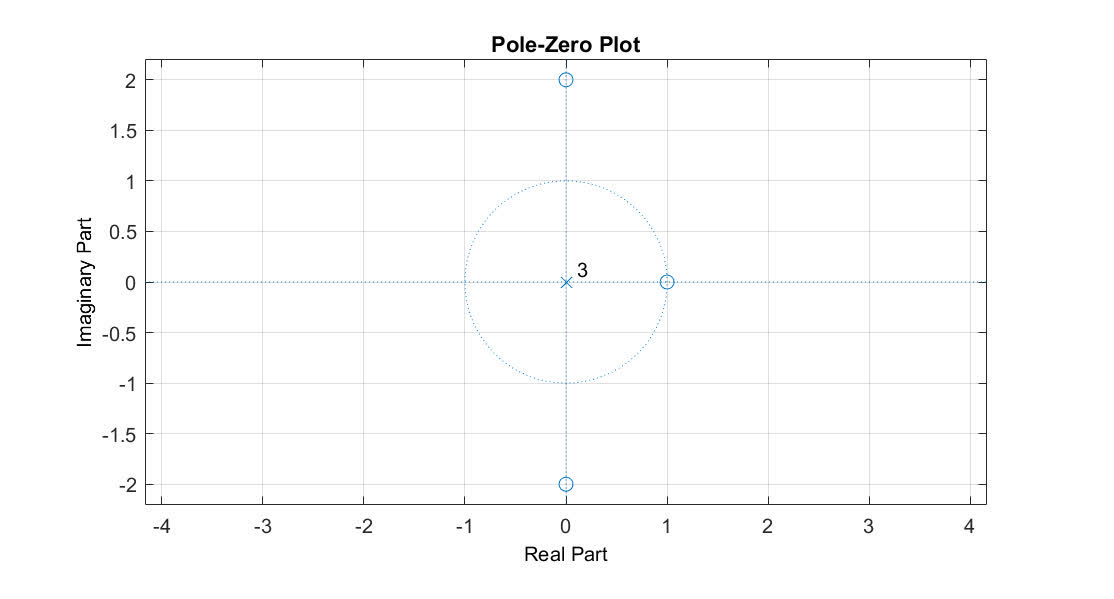
\includegraphics[width=1\textwidth]{images/20220217_01.png}
        \end{center}
        For the amplitude we just look at the pole-zero plot and multiply all origin-zero distances while we divide for all origin-pole distances. As all the poles are at the origin, their distance from a point on the circle will always be 1. We plot from 0 to $\pi$ as $-\pi$ to $0$ is symmetric, so normalized in $0$ to $1$. As $z=\rho e^{j2\pi f}=e^{j\omega}$:
        \begin{itemize}
            \item $\omega=0,\,\,z=0\rightarrow|H(z)|=0$
            \item $\omega=\frac{\pi}{2},\,\,z=j\rightarrow|H(z)|=3\sqrt{2}\sim 4.24$
            \item $\omega=\pi,\,\,z=-1\rightarrow|H(z)|=2\sqrt{5}\sqrt{5}=10$
        \end{itemize}
    }

    \mybox{
        \begin{center}
            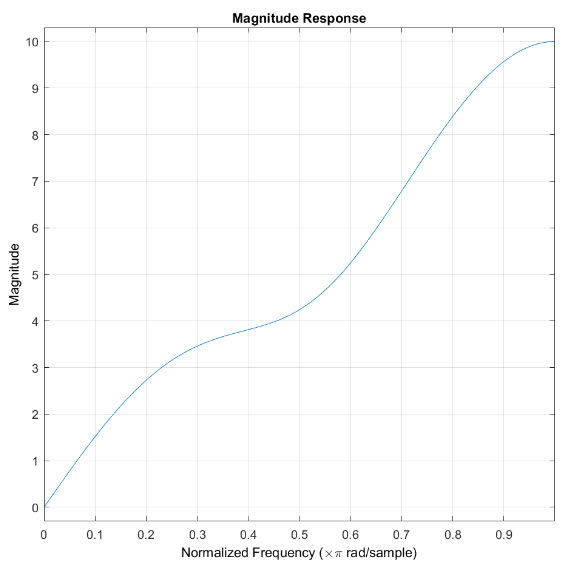
\includegraphics[width=0.8\textwidth]{images/20220217_12.png}
        \end{center}
    }

    \subsubsection{Define minimum phase filter with fixed amplitude}
    [2 pts] In case of it is a maximum phase filter provide its minimum phase version with the same magnitude response otherwise, if it is a "minimum phase filter" provide its maximum phase version.

    \mybox{
        Write the $G$ version of those that introduce maximum phase:
        $$
        H(z)=1-z^{-1}+4z^{-2}-4z^{-3}=(z^{-1}-1)(-4z^{-2}-1)=(1-z^{-1})(1+4z^{-2})
        $$
        $$
        \begin{cases}
            \rho^2=4\\
            2\rho\cos\theta=0
        \end{cases}
        \Rightarrow
        \begin{cases}
            \rho=2\\
            \theta=\pm\frac{\pi}{2}
        \end{cases}
        $$
        Write the $G$ version of those that introduce maximum phase:
        $$
        H_m(z)=(1-z^{-1})(4+z^{-2})=4-4z^{-1}+z^{-2}-z^{-3}
        $$
    }

    \subsubsection{Output samples: convolution}
    [3 pts] Working in the time domain evaluate the output $y[n]$ of the signals
    $x_a[n]=\Brackets{1,-1,1,-1}$ and $x_b[n]=\Brackets{1,1,1,1}$ with filter $h[n]$.

    \mybox{
        $$h[n]=\delta(n)-\delta(n-1)+4\delta(n-2)-4\delta(n-3)$$
        \begin{center}
            \begin{tabular}{c|c c c c c c c}
                $n=$        & 0 & 1 &  2 &  3 & 4 & 5 & 6\\ \hline \hline
                $x_a[n]$    & 1 & -1 & 1 & -1\\
                $-x_a[n-1]$ &  0 & -1 & 1 & -1 & 1\\
                $4x_a[n-2]$ &  0 &  0 & 4 & -4 & 4 & -4\\
                $-4x_a[n-3]$&  0 &  0 & 0 &-4 &  4 &-4 & 4\\ \hline
                $y_a[n]$    &  1 & -2 & 6 &-10& 9 & -8 & 4
            \end{tabular}        
        \end{center}
        \vspace{1em}
        \begin{center}
            \begin{tabular}{c|c c c c c c c}
                $n=$        & 0 & 1 &  2 &  3 & 4 & 5 & 6\\ \hline \hline
                $x_b[n]$    & 1 &  1 & 1 &  1\\
                $-x_b[n-1]$ & 0 & -1 &-1 & -1 &-1\\
                $4x_b[n-2]$ & 0 &  0 & 4 &  4 & 4 & 4\\
                $-4x_b[n-3]$& 0 &  0 & 0 & -4 &-4 &-4 &-4\\ \hline
                $y_b[n]$    & 1 &  0 & 4 &  0 &-1 & 0 &-4
            \end{tabular}        
        \end{center}
    }

\pagebreak\subsection{20220217-2*}
    A signal $x(t)=\sin(2\pi 100t)+2\cos(2\pi 50t)$ is sampled at $400Hz$ and then downsampled by an order of $M=3$

    \subsubsection{Downsampling without LPF}
    [5pts] What is the output in case of no low pass (antialiasing) filter is adopted? Depict the magnitude of the output in the range $0-\pi$ (normalized frequencies).

    \mybox{
        $$
        F_s=400
        $$
        The sampled signal is
        $$
        x[n]=\sin(\frac{\pi}{2}n)+2\cos(\frac{\pi}{4}n)
        $$
        So after downsampling:
        $$
        x_d[n]=x[nM]=\sin(\frac{3\pi}{2}n)+2\cos(\frac{3\pi}{4}n)
        $$

    }

\pagebreak\subsection{20220126-1}
    We need to apply the first derivative ($h[n]=\Brackets{1,-1}$) in real-time to a digital signal $x[n]=\Brackets{1,2,0,1,0,1,\cdots}$ working in the frequency domain on blocks of 4 samples.

    \subsubsection{DFT}
    [4pts] Describe how to get the DFT for each block of the signal and for the filter according to the requested task.

    \mybox{
        Just use the $W$ matrix of dimension 4:
        $$
        W=
        \begin{bmatrix}
            1 & 1 & 1 & 1\\
            1 & -j & -1 & j\\
            1 & -1 & 1 & -1\\
            1 & j & -1 & -j
        \end{bmatrix}
        $$
        So the DFT of the filter will be:
        $$
        H[k]=
        \begin{bmatrix}
            1 & 1 & 1 & 1\\
            1 & -j & -1 & j\\
            1 & -1 & 1 & -1\\
            1 & j & -1 & -j
        \end{bmatrix}
        \begin{bmatrix}
            1\\
            -1\\
            0\\
            0
        \end{bmatrix}=
        \begin{bmatrix}
            0\\
            1+j\\
            2\\
            1-j
        \end{bmatrix}
        $$
    }

    \subsubsection{Overlap and save}
    [7pts] Using the overlap and save algorithm, describe how to find the output for the given signal, provide all the intermediate numerical results and the steps to obtain the final result.

    \mybox{
        Blocks of 4 samples, for overlap and save fot the first block we add $\underlabel{P}{len(h)}-1=1$ leading zeros:
        \vspace{1em}

        $
        x_1[n]=\Brackets{0,1,2,0}\\
        \\
        x_2[n]=\Brackets{0,-1,0,1}\\
        $

        \vspace{1em}
        At this point we could circular convolve with the filter then DFT, or we first DFT the blocks then circular convolve. We decide the first approach and we will get (as $h[n]=\delta[n]-\delta[n-1]$)

        $
        y_1[n]=\Brackets{0,1,1,-2,0}
        $
    }

\pagebreak\subsection{20211108-1}

    \subsubsection{Zero-pole to equation in z}

    \mybox{
        $$
        H_m(z)=1+0.49z^{-2}
        $$
    }

\pagebreak\subsection{20190910-2}
    A signal $x[n]=\Brackets{-1,-1,2,0,0,1,-2,1,0,1,1,-1}$ shall be filtered with this FIR fitler: $h[n]=\Brackets{1,-1,2}$.\\
    We need to process blocks of 4 samples of the original signal for real time processing and we want to get the result depicting all intermediate steps with these methods:

    \subsubsection{Overlap and Add}
    [4pt] Overlap and Add

    \mybox{
        Subdividing the signal in blocks of $L$ elements, in this case $L=N=4$ so we get 3 blocks:
        \vspace{1em}

        $
        x_1[n]=\Brackets{-1,-1,2,0}\\
        x_2[n]=\Brackets{0,1,-2,1}\\
        x_3[n]=\Brackets{0,1,1,-1}
        $

        \vspace{1em}
        Now we filter using convolution with $h[n]=\Brackets{1,-1,2}$
        \vspace{1em}

        $
        x[n]*h[n]=x[n]*\delta[n]+x[n]*-\delta[n-1]+x[n]*2\delta[n-2]=\\
        =\cdots x[n]-x[n-1]+2x[n-2]=\\
        $

        \begin{center}
            \begin{tabular}{c|c c c c c c}
                $n=$        & 0 & 1 &  2 &  3 & 4 & 5\\ \hline \hline
                $x_1[n]$    & -1 & -1 & 2 & 0\\
                $-x_1[n-1]$ &  0 &  1 & 1 & -2 & 0\\
                $2x_1[n-2]$ &  0 &  0 &-2 & -2 & 4 & 0\\ \hline

                $x_2[n]$    & 0 & 1  & -2 & 1\\
                $-x_2[n-1]$ & 0 &  0 & -1 & 2 &-1\\
                $2x_2[n-2]$ & 0 &  0 & 0  & 2 &-4 & 2\\ \hline

                $x_3[n]$    & 0 &  1 & 1 & -1\\
                $-x_3[n-1]$ & 0 &  0 &-1 & -1 & 1\\
                $2x_3[n-2]$ & 0 &  0 & 0 & 2  & 2 & -2

            \end{tabular}        
        \end{center}
        \vspace{1em}

        $
        \Rightarrow y_1[n]=\begin{Bmatrix}
            -1 & 0 & 1 & -4 & 4 & 0
        \end{Bmatrix}\\
        \Rightarrow y_2[n]=\begin{Bmatrix}
            0 & 1 & -3 & 5 & -5 & 2
        \end{Bmatrix}\\
        \Rightarrow y_3[n]=\begin{Bmatrix}
            0 & 1 & 0 & 0 & 3 & -2
        \end{Bmatrix}
        $

        \vspace{1em}
        Considering the overlapping tails, as:
        $$
        y[n]=x[n]*h[n]=\sum_{r=0}^\infty y_r[n-r\underlabel{L}{4}]
        $$
        $$
        \begin{bmatrix}
            -1 & 0 & 1 &-4 & 4 & 0\\
            &   &   &   & 0 & 1 &-3 & 5 &-5 & 2\\    
            &   &   &   &   &   &   &   & 0 & 1 & 0 & 0 & 3 & -2\\    
        \end{bmatrix}
        $$
        And the final result is
        $$
        y[n]=\begin{Bmatrix}
            -1 & 0 & 1 & -4 & 4 & 1 & -3 & 5 & -5 & 3 & 0 & 0 & 3 & -2
        \end{Bmatrix}
        $$
    }
    \subsubsection{Overlap and Save}
    [4pt] Overlap and Save

    \mybox{
        Subdividing the signal in blocks of $L$ elements, in this case $L=N=4$ so we get 3 blocks:
        \vspace{1em}

        $
        x_1[n]=\Brackets{-1,-1,2,0}\\
        x_2[n]=\Brackets{0,1,-2,1}\\
        x_3[n]=\Brackets{0,1,1,-1}
        $

        \vspace{1em}
        As the filter $h[n]$ has length $P=3$, we need to add $P-1=2$ "0"s at the beginning to account for the circular convolution effect, and for each $x_{i>1}$ we add the 2 samples before, hence in overlap and save
        $$L=N+P-1=4+2=6$$

        $
        x_1[n]=\Brackets{\mathbf{0,0,}-1,-1,2,0}\\
        x_2[n]=\Brackets{\mathbf{2,0,}0,1,-2,1}\\
        x_3[n]=\Brackets{\mathbf{-2,1,}0,1,1,-1}
        $

        \vspace{1em}
        Now we filter using circular convolution with $h[n]=\Brackets{1,-1,2}$. But we don't compute the circular convolution traditionally, we use this strategy:
        $$x_L\circledast h_L=\left[\underlabel{\cdots\cdots}{$P-1$ to discard}\cdots\cdots\underlabel{\cdots}{$L-1$}\right]$$
        a circular convolution of block $L$ will discard the first $P-1$ samples, then the rest till $L-1$ will be the same obtained from a normal convolution
        $$
        x[n]*h[n]=x[n]*\delta[n]+x[n]*-\delta[n-1]+x[n]*2\delta[n-2]=x[n]-x[n-1]+2x[n-2]
        $$

        \begin{center}
            \begin{tabular}{c|c c c c c c}
                $n=$        & 0 & 1 &  2 &  3 & 4 & 5\\ \hline \hline
                $x_1[n]$    & 0 & 0 & -1 & -1 & 2 & 0\\
                $-x_1[n-1]$ & 0 & 0 &  0 &  1 & 1 & -2\\
                $2x_1[n-2]$ & 4 & 0 &  0 &  0 &-2 & -2\\ \hline

                $x_2[n]$    & 2 & 0  & 0 & 1  & -2 & 1\\
                $-x_2[n-1]$ &-1 & -2 & 0 &  0 & -1 & 2\\
                $2x_2[n-2]$ &-4 & 2  & 4 &  0 & 0  & 2\\ \hline

                $x_3[n]$    & -2 & 1 & 0 &  1 & 1 & -1\\
                $-x_3[n-1]$ & 1  & 2 &-1 &  0 &-1 & -1\\
                $2x_3[n-2]$ & 2  &-2 &-4 &  2 & 0 & 2

            \end{tabular}        
        \end{center}
        \vspace{1em}
        We throw the first two as $P-1=2$, so:
        \vspace{1em}

        $
        \Rightarrow y_1[n]=\begin{Bmatrix}
            \cdot & \cdot & -1 & 0 & 1 & 4
        \end{Bmatrix}\\
        \Rightarrow y_2[n]=\begin{Bmatrix}
            \cdot & \cdot & 4 & 1 & -3 & 5
        \end{Bmatrix}\\
        \Rightarrow y_3[n]=\begin{Bmatrix}
            \cdot & \cdot & -5 & 3 & 0 & 0
        \end{Bmatrix}
        $

        \vspace{1em}
        And the final result is
        $$
        y[n]=\Brackets{y_1\,\,y_2\,\,y_3}=\begin{Bmatrix}
            -1 & 0 & 1 & 4 & 4 & 1 & -3 & 5 & -5 & 3 & 0 & 0
        \end{Bmatrix}
        $$
    }




% \begin{center}
%     \begin{tabular}{X|c c c c c c}
%         $n=1$       & 0 & 1 &  2 &  3 & 4 & 5\\ \hline
%         $x_1[n]$    & 0 & 0 & -1 & -1 & 2 & 0\\
%         $-x_1[n-1]$ & 0 & 0 &  0 &  1 & 1 & -2\\
%         $2x_1[n-2]$ & 0 & 0 &  0 &  0 &-2 & -2
%     \end{tabular}        
% \end{center}

\pagebreak\subsection{20190722-1}
    A signal $x(t)$ is sampled at $10kHz$, and we want to find the relative magnitude of its components at $1kHz$ w.r.t. the components at $4kHz$ but we \underline{cannot} use the FFT.

    Therefore we decide to filter the signal at $1kHz$ and $4kHz$ multiplying it with a real sinusoid at $1kHz$ and at $4kHz$ respectively.

    \subsubsection{Not using FFT/DFT, use a cosine and pole-zero plot}
    [3 pts] Depict the pole zero plots for the two sinusoids.

    \mybox{
        The signal is sampled at $10kHz$ so
        $$F_s=10kHz$$
        If we could use th DFT or FFT, we could just use
        $$
        X(k)=\sum_{n=0}^{N-1} x(n)e^{-j2\pi \frac{k}{N}n}\big|_{f=1kHz}
        $$
        Instead we exploit a real sinusoid in the time domain:
        $$
        s(n)=\cos(2\pi \overline{f}n)
        $$
        Whose Fourier transform will result in two pulses (two $\delta$'s) in the frequency domain as it is a cosine: in $\overline{f}$ and in $-\overline{f}$. If we compute
        $$
        X(f)\cdot DTFT(\cos(2\pi fn))\big|_{f=1kHz}=X(f=1kHz)\delta(f-1kHz)+X(f=1kHz)\delta(f+1kHz)
        $$
        As we consider normalized frequencies and compute the z-transform:
        $$f_1=1kHz\rightarrow \tilde{f}_1=\frac{f_1}{Fs}$$
        $$
        \cos\left(2\pi\frac{1kHz}{10kHz}n\right)\cdot\underlabel{u(n)}{Discrete unitary step, the signal is defined only in the positive values}
        $$
        Using
        $$
        Z\brackets{r^n\cos(\omega_0n)u(n)}=\frac{1-r\cos(\omega_0)z^{-1}}{1-2r\cos(\omega_0)z^-1+r^2z^{-2}}
        $$
        $$
        Z-TX=\frac{1-\cos(\bigslant{\pi}{5})z^{-1}}{
            1-2\cos(\bigslant{\pi}{5})z^{-1}+z^{-2}}
        $$
    }

    \mybox{
        Alternatively we convert it to the exponential form and solve the z-transform explicitely
        $$
        \begin{cases}
            \frac{e^{j\frac{\pi}{5}n}+e^{-j\frac{\pi}{5}n}}{2}\cdot u(n)\\
            X(z)=\sum_{n=-\infty}^{+\infty}x(n)\cdot z^{-n}
        \end{cases}
        $$
        So due to geometric sum:
        $$
        Z-TX(e^{j\frac{\pi}{5}n}\cdot u(n))=\sum_{n=0}^\infty e^{j\frac{\pi}{5}n}z^{-n}=\sum_{n=0}^\infty\left(e^{j\frac{\pi}{5}}z^{-1}\right)^n=\frac{1}{1-e^{j\frac{\pi}{5}z^{-1}}}
        $$
        $$
        Z-TX=\frac{1}{2}\left(\frac{1}{1-e^{j\frac{\pi}{5}z^{-1}}}+\frac{1}{1-e^{-j\frac{\pi}{5}z^{-1}}}\right)=\cdots
        $$
        From
        $$
        H_1(z)=\frac{1-\cos(\bigslant{\pi}{5})z^{-1}}{1-2\cos(\bigslant{\pi}{5})z^{-1}+z^{-2}}
        $$
        We can find the zeros and the poles
        \begin{itemize}
            \item For the denominator we exploit:
            $$
            1-2\rho\cos(\theta)z^{-1}+\rho^2z^{-2}\leftrightarrow \rho(\cos(\theta)\pm j\sin(\theta))
            $$
            Poles in $e^{\pm j\frac{\pi}{5}}$ \textbf{plus double zero in the origin}
            \item For the numerator the zeros are just the coefficients of $z^{-k}$, so we have a zero in $\cos(\frac{\pi}{5})$ \textbf{plus a pole in the origin which will cancel out with the double zero in the origin leaving a single zero}
        \end{itemize}
        \begin{center}
            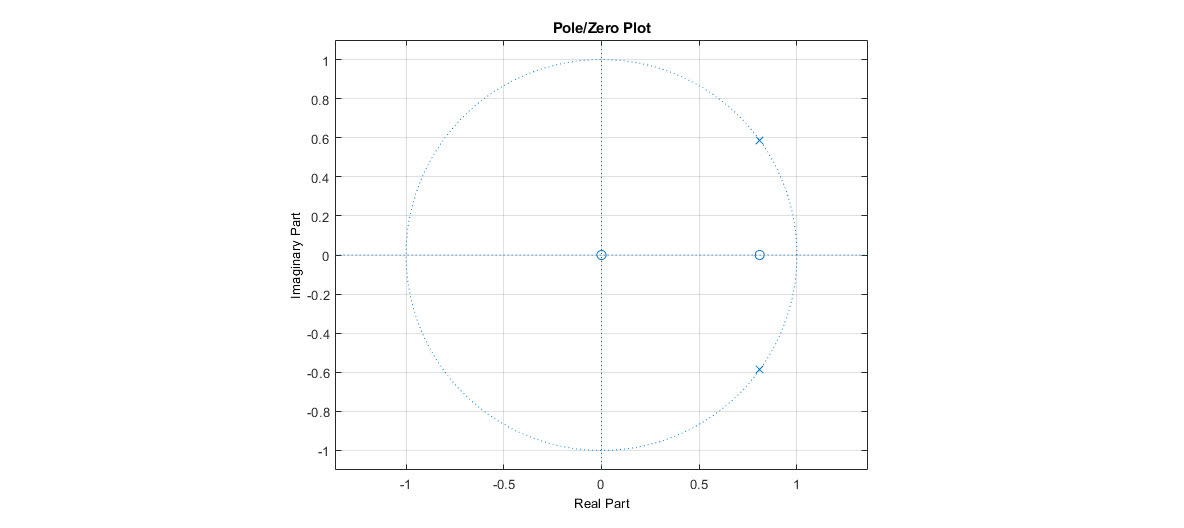
\includegraphics[width=1\textwidth]{images/20190722_01.png}
        \end{center}
        Same reasoning for $4Hz$, we will get
        $$
        H_2(z)=\frac{1-\cos(\bigslant{4\pi}{5})z^{-1}}{1-2\cos(\bigslant{4\pi}{5})z^{-1}+z^{-2}}
        $$
    }

    \subsubsection{Difference equations (anti z-transform)}
    [6 pts] Define the difference equations both for the first and the second sinusoid.

    \mybox{
        Everything at numerator will be $x$'s on the right, everything at the denominator will be $y$'s on the left:
        \vspace{1em}

        $
        H_1(z)=\frac{1-\cos(\bigslant{\pi}{5})z^{-1}}{1-2\cos(\bigslant{\pi}{5})z^{-1}+z^{-2}}\\
        \\
        y_1(n)-2\cos(\bigslant{\pi}{5})y(n-1)+y(n-2)=
        1-\cos(\bigslant{\pi}{5})x(n-1)\\
        \\
        H_2(z)=\frac{1-\cos(\bigslant{4\pi}{5})z^{-1}}{1-2\cos(\bigslant{4\pi}{5})z^{-1}+z^{-2}}\\
        \\
        y_2(n)-2\cos(\bigslant{4\pi}{5})y(n-1)+y(n-2)=
        1-\cos(\bigslant{4\pi}{5})x(n-1)\\
        $
    }

    \subsubsection{How to apply the filters}
    [3 pts] Describe how we shall apply the previously defined filters in order to measure the relative intensity of the input signal at 1kHz with respect to 4kHz.

    \mybox{
        In order to apply the filters we have to take a portion of the input signal and process it with the two filters (the difference equations above).
        
        To avoid polarizations in the measure we should take a set of samples multiple of the wavelengths (in term of samples) of both the sinusoids. 
        
        The ratio of the two magnitudes of the outputs will give the result.
    }

    \subsubsection{Cosine method weakness w.r.t. Fourier Transform}
    [1 pts] What is a weakness of the proposed system with respect to the Fourier Transform?

    \mybox{
        The weakness with respect to the Fourier Transform is related to the fact that we are not using the phase as in the Discrete Fourier Transform, so, signal components with the same amplitude and frequency but different phases will give different results.

        By multiplying our signal with a signal in the Fourier domain, it means that we are convolving the signal with a cosine:
        $$
        y(n)=\sum_mx(n-m)\cos(2\pi\underlabel{\tilde{f}}{1kHz}n)
        $$
        While the DFT:
        $$
        X(k)=\sum_{n=0}^{N-1} x(n)e^{-j2\pi \frac{k}{N}n}\big|_{f=1kHz}=
        \sum_{n=0}^{N-1} x(n)\left(\cos(2\pi fn)-j\sin(2\pi fn)\right)\big|_{f=1kHz}
        $$
        So we are not considering a sin component.
    }

\pagebreak\subsection{20190212-2}
    A signal is sampled at $10kHz$ filling all the available band. We need to upsample it to $15kHz$.

    \subsubsection{Upsample by noninteger pipeline}
    [3pts] Provide the full pipeline to properly upsample the signal minimizing the presence of artifacts or aliasing and detailing the parameters of every bock

    \mybox{
        As we upsample to a noninteger, we can:
        $$10\rightarrow 30\rightarrow 15$$
        So we first upsample by $L=3$ and then downsample by $M=2$, which means we introduce a LPF of $\Omega_c=\min\left(\frac{\pi}{3},\frac{\pi}{2}\right)=\frac{\pi}{3}$ (in other words a filter with that cutoff $H(z)\big|_{\omega_c=\frac{\pi}{3},f_c=\frac{1}{6}}$)
        \begin{center}
            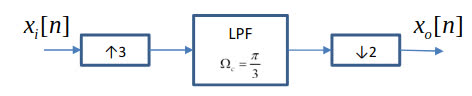
\includegraphics[width=0.8\textwidth]{images/20190212_21.png}
        \end{center}
    }

    \subsubsection{Cutoff DFT}
    [7pts] Assuming that we are working on blocks of 8 samples and we are filtering the signal in frequency domain, describe a possible implementation of the previous system working in the frequency domain (using the DFT).

    \mybox{
        8 samples, so $N=8$, after upsample we will have $8\cdot 3=24$ samples. If we have to implement that filter with that frequency and 24 samples, so
        $$
        f=\left[
            0,\frac{1}{24},\frac{2}{24},\cdots,\frac{23}{24}
        \right]
        $$
        24 samples that represent normalized frequencies, a cutoff of $f_c=\frac{1}{6}$ means that we keep the pulses till $f_c$ and introduce at the end 3 pulses (symmetry)
        \begin{center}
            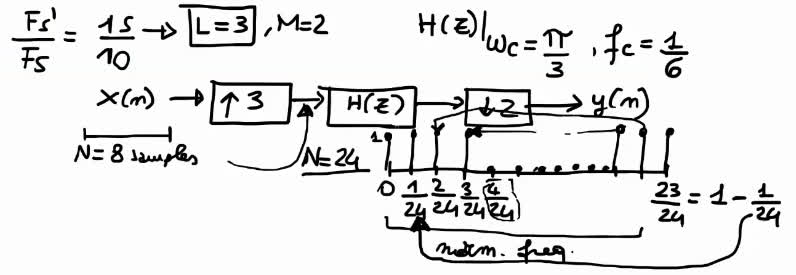
\includegraphics[width=1\textwidth]{images/20190212_22.png}
        \end{center}
    }

\pagebreak\subsection{20190116-2}
    A maximum phase filter has the following transfer function:
    $$
    H_M(z)=\frac{
        \left(
            1-2\sqrt{2}z^{-1}+4z^{-2}
        \right)
        \left(
            1+2\sqrt{2}z^{-1}+4z^{-2}
        \right)
    }{4+z^{-2}}
    $$

    \subsubsection{Zero-pole plot}
    [2 Pts.] Provide its zeros-poles plot

    \mybox{
        Poles:
        $$z^{-2}=-4\rightarrow \pm\frac{i}{2}$$
        Zeros, make sure the $\Delta<0$, otherwise we cannot use the formula for complex conjugates. In this case the condition holds, so
        $$
        1-2\rho\cos\theta z^{-1}+\rho^2 z^{-2}
        \Rightarrow
        \begin{cases}
            2\sqrt{2}=2\rho\cos\theta\\
            4=\rho^2
        \end{cases}\Rightarrow
        \begin{cases}
            \rho=2\\
            \theta=\pm\frac{\pi}{4}
        \end{cases}
        $$
        $$
        1-2\rho\cos\theta z^{-1}+\rho^2 z^{-2}
        \Rightarrow
        \begin{cases}
            -2\sqrt{2}=2\rho\cos\theta\\
            4=\rho^2
        \end{cases}\Rightarrow
        \begin{cases}
            \rho=2\\
            \theta=\pm\frac{3}{4}\pi
        \end{cases}
        $$
        We also introduced in the origin 2 zeros and 4 poles, so we will have 2 poles:
        \begin{center}
            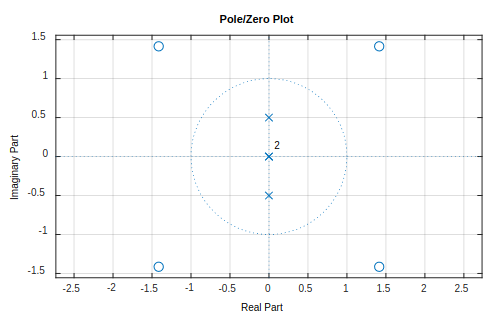
\includegraphics[width=0.7\textwidth]{images/20190116_21.png}
        \end{center}
    }

    \subsubsection{Define minimum phase filter with fixed amplitude/magnitude}
    [4 Pts.] Provide its minimum phase version, $H_m(z)$, with exactly the same magnitude response.

    \mybox{
        As $\rho=2$, now $\rho=\frac{1}{2}$:
        $$
        H_m(z)=A\frac{
            \left(
                1-\frac{\sqrt{2}}{2}z^{-1}+\frac{1}{4}z^{-2}
            \right)
            \left(
                1+\frac{\sqrt{2}}{2}z^{-1}+\frac{1}{4}z^{-2}
            \right)
        }{4+z^{-2}}
        $$
    }

    \mybox{
        Then we find $A$ by imposing:
        $$H_M(z=0)=H_m(z=0)\Rightarrow \frac{1}{4}=A\frac{1}{4}\Rightarrow A=16$$
        Alternatively write the $G$ version of those that introduce maximum phase
        $$
        H_m(z)=\frac{
            \left(
                4-2\sqrt{2}z^{-1}+z^{-2}
            \right)
            \left(
                4+2\sqrt{2}z^{-1}+z^{-2}
            \right)
        }{4+z^{-2}}
        $$
    }

    \subsubsection{Cosine signal and generic filter}
    [5 Pts.] A signal $x(t)=\cos(2\pi 1000t)$ is sampled at $4kHz$. Define the outputs $y_M[n]$ and $y_m[n]$ with the proper amplitude and phase from the two filters $H_M(z)$ and $H_m(z)$.

    \mybox{
        A cosine by a generic filter $H$ will give another cosine with different amplitude and phase.

        $f_0=1000=1kHz$, $F_s=4kHz$, so the normalized frequency $\tilde{f}_0=\frac{f_0}{F_s}=\frac{1}{4}$ and $\tilde{\omega}_0=\frac{\pi}{2}$

        In the z-transform we will have (we always consider the normalized!):
        $$
        z_0=1*e^{j\omega}=e^{j2\pi f}=e^{j\pi/2}=j
        $$
        \begin{itemize}
            \item Maximum phase
            $$
            H_M(z)\rightarrow\begin{cases}
                \left|H_M(z=j)\right|=\cdots=\frac{17}{3}\\
                \angle H_M(z=j)=\angle
                H_M(z)=\frac{
                    \left(
                        1-2\sqrt{2}j^{-1}-4
                    \right)
                    \left(
                        1+2\sqrt{2}j^{-1}-4
                    \right)
                }{4-1}
            \end{cases}
            $$
            The phase:
            $$
            \angle
                H_M(z)=\frac{
                    \left(
                        2\sqrt{2}j-3
                    \right)
                    \left(
                        -2\sqrt{2}j-3
                    \right)
                }{3}
                =
                \angle(-3+2\sqrt{2}j)+\angle(-3-2\sqrt{2}j)+\angle(3)
            $$
            The phase of a real number is zero in the complex plane, while the phase of the first term will be in the third quadrant and the phase of the second term will be the first mirrored, so summing them together will get $\angle H_M(j)=2\pi$
            $$y_M(n)=A\cdot\cos(\tilde{\omega}_0n+\phi)=\frac{17}{3}\cos(\frac{\pi}{2}n+2\pi)$$
            \item Minimum phase, as we \textbf{imposed that the magnitude is the same}
            $$
            H_m(z)\rightarrow\begin{cases}
                \left|H_m(z=j)\right|=\left|H_M(z=j)\right|=\frac{17}{3}\\
                \angle H_M(z=j)=\angle
                \frac{
                    \left(
                        3+2\sqrt{2}j
                    \right)
                    \left(
                        3-2\sqrt{2}j
                    \right)
                }{3}
                =
                0
            \end{cases}
            $$
            The phase is 0 as the phase of the first is in the first quadrant $\angle H_m(j)=0$
            $$y_m(n)=A\cdot\cos(\tilde{\omega}_0n+\phi)=\frac{17}{3}\cos(\frac{\pi}{2}n+0)$$
        \end{itemize}
    }

\pagebreak\subsection{20181107-1}
    An analog signal $x(t)=2\cos(2\pi 20t)+3\sin(2\pi 60t)+4\cos(2\pi 80t)$ is sampled at 160 samples/s and filtered with an IIR filter with the following finite differences equation:
    $$
    y[n]=x[n]+\sqrt{2}x[n-1]+x[n-2]-0.9\sqrt{2}[n-1]-0.81y[n-2]
    $$

    \subsubsection{Z-transform and pole-zero plot}
    [2pts] Provide the z-transform of the filter.

    [3pts] Provide the zeros-poles plot of the filter.

    \mybox{
        $$F_s=160$$
        So the sampled signal is
        $$
        x(t)=2\sin(\frac{\pi}{4} n)+3\cos(\frac{3\pi}{4}n)+4\sin(\pi n)
        $$
        $$
        H(z)=\frac{
            1+\sqrt{2}z^{-1}+z^{-2}
        }{
            1+0.9\sqrt{2}z^{-1}+0.81z^{-2}
        }
        $$
        \begin{itemize}
            \item Numerator:
            $$
            \begin{cases}
                \rho^2=1\\
                2\rho\cos\theta=-\sqrt{2}
            \end{cases}
            \Rightarrow
            \begin{cases}
                \rho=1\\
                \theta=\pm\frac{3\pi}{4}
            \end{cases}
            $$
            Two zeros in $e^{\pm j\frac{3\pi}{4}}$, two poles in 0
            \item Denominator:
            $$
            \begin{cases}
                \rho^2=0.81\\
                2\rho\cos\theta=-0.9\sqrt{2}
            \end{cases}
            \Rightarrow
            \begin{cases}
                \rho=0.9\\
                \theta=\pm\frac{3\pi}{4}
            \end{cases}
            $$
            Two poles in $0.9e^{\pm j\frac{3\pi}{4}}$, two zeros in 0
        \end{itemize}
        So no zeros or poles at the origin, system stable as all poles and zero in the circle:
        \begin{center}
            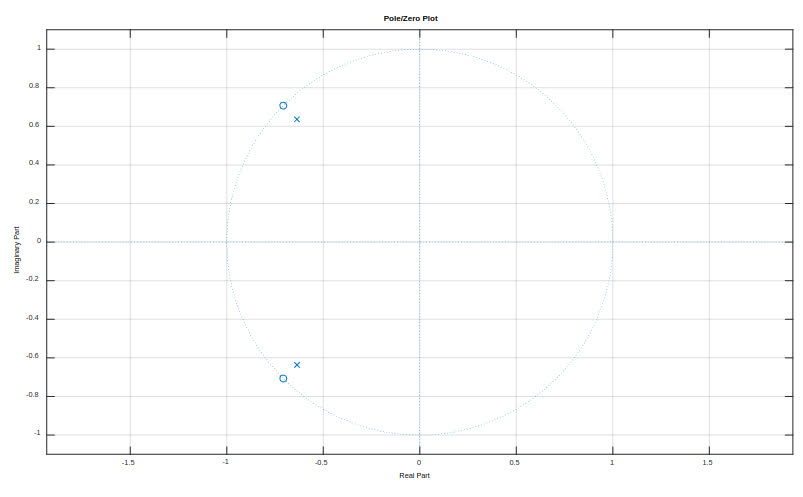
\includegraphics[width=0.9\textwidth]{images/20181107_11.png}
        \end{center}
    }

    \subsubsection{Magnitude and phase plot by hand}
    [3pts] Represent an approximate behavior of the magnitude and phase in the range $(0\,\,-\pi)$.

    \mybox{
        $$
        H(z)=\frac{
            1+\sqrt{2}z^{-1}+z^{-2}
        }{
            1+0.9\sqrt{2}z^{-1}+0.81z^{-2}
        }
        $$
        The range is normalized in $(0\,\,1)$. We start from the magnitude, we compute some notable points:
        \begin{itemize}
            \item $|H(z=1,\omega=0)|=\frac{2+\sqrt{2}}{1.81+0.9\sqrt{2}}\sim 1.1075$
            \item $|H(z=j,\omega=\pi/2)|=\left|\frac{-\sqrt{2}j}{0.19-0.9\sqrt{2}j}\right|=\frac{\sqrt{2}}{\sqrt{0.19^2+0.81*2}}\sim 1.0989$
            \item $|H(z=e^{-j\frac{3\pi}{4}},\omega=3\pi/4)|=0$, as in that angle we meet the zero so we are multiplying by 0
            \item $|H(z=-1,\omega=\pi)|=\frac{2-\sqrt{2}}{1.81-0.9\sqrt{2}}\sim 1.0904$
        \end{itemize}
        \begin{center}
            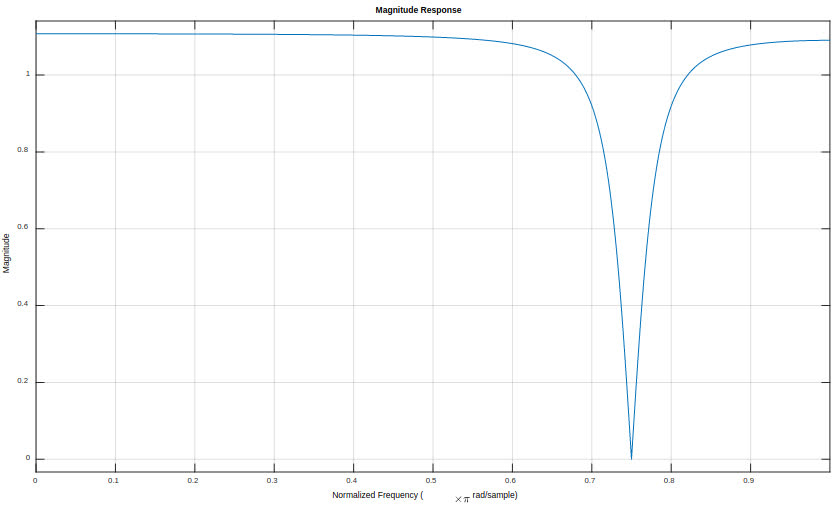
\includegraphics[width=0.8\textwidth]{images/20181107_12.png}
        \end{center}

        About the phase, we have to look at the zero plot:
        \begin{itemize}
            \item $\angle H(z=1)=0$ as we have opposite contributes for both poles and zeros
            \item $\angle H(z=e^{-j\frac{3\pi}{4}})$ we don't know the exact value, but at that pole we will have a jump of $\pi$
            \item $\angle H(z=-1)=0$ as we have opposite contributes for both poles and zeros
        \end{itemize}
        \begin{center}
            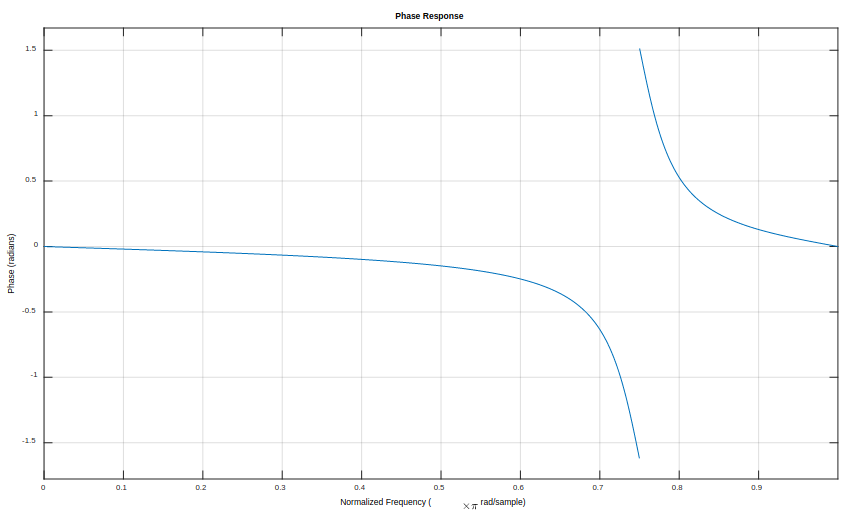
\includegraphics[width=0.8\textwidth]{images/20181107_13.png}
        \end{center}
    }

    \subsubsection{Sampled signal, cosine signal and generic filter}
    [5pts] What will be the discrete output signal when the input is the sampled version of $x(t)$

    \mybox{
        $$F_s=160$$
        The signal is
        $$
        x(t)=2\cos(2\pi 20t)+3\sin(2\pi 60t)+4\cos(2\pi 80t)
        $$
        It has three components, so:
        \begin{itemize}
            \item $\tilde{f_1}=\frac{f_1}{F_s}=\frac{20}{160}=\frac{1}{8}\rightarrow\tilde{\omega}_1=\frac{\pi}{4}\rightarrow z_1=1*e^{j\pi/4}$
            $$
            \begin{cases}
                |H(z_1)|=\cdots=1.1068\\
                \angle H(z_1)=\cdots=-0.053
            \end{cases}
            $$
            \item $\tilde{f_2}=\frac{f_2}{F_s}=\frac{60}{160}=\frac{3}{8}\rightarrow\tilde{\omega}_2=\frac{3\pi}{4}\rightarrow z_2=1*e^{j3\pi/4}$
            $$
            \begin{cases}
                |H(z_2)|=0\\
                \angle H(z_2)=\text{ does not matter, the magnitude is 0 so the term disappears}
            \end{cases}
            $$
            \item $\tilde{f_3}=\frac{f_3}{F_s}=\frac{80}{160}=\frac{1}{2}\rightarrow\tilde{\omega}_3=\pi\rightarrow z_3=1*e^{j\pi}=-1$
            $$
            \begin{cases}
                |H(z_3)|=1.0904\\
                \angle H(z_3)=0
            \end{cases}
            $$
        \end{itemize}
        The output is:
        $$
        y[n]=2\cdot 1.1065\cos\left(\frac{\pi}{4}n-0.053\right)+4\cdot 1.09\cos(\pi n)
        $$
    }

\pagebreak\subsection{20160223-1}
    A filter $H_1(z)$ presents the following zero-pole plot:
    \begin{center}
        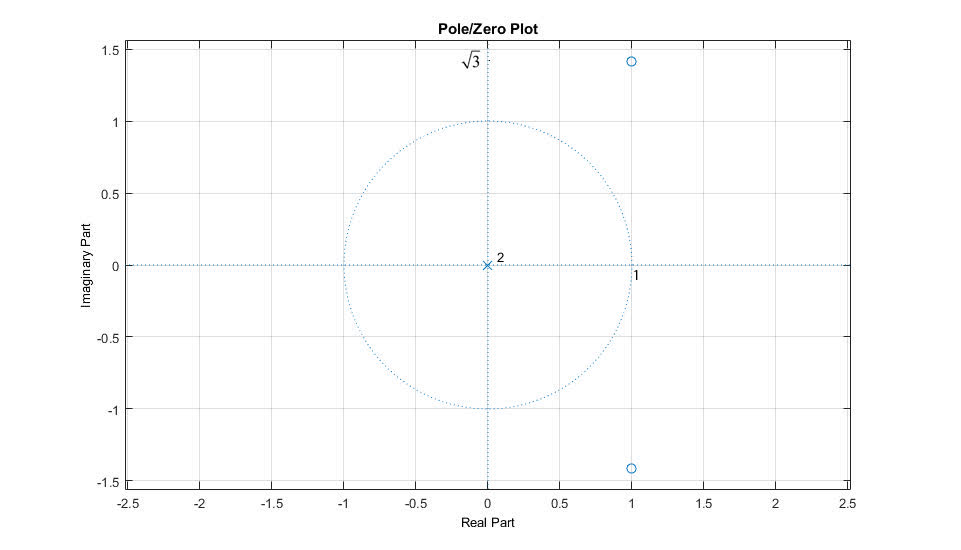
\includegraphics[width=1\textwidth]{images/20160223_01.png}
    \end{center}
    Where the two zeros are in $1\pm\sqrt{3}j$

    \subsubsection{Define minimum phase filter with fixed amplitude}
    Define a minimum phase filter $H_2(z)$ with \textbf{exactly} the same amplitude response

    \mybox{
        As two zeros are outside, we are dealing with maximum phase filter: we want to bring the zeros inside keeping the same amplitude, so we must \textbf{move zeros to their complex conjugate position, inside the circle}.\\
        For example the zero on top-right has distance $\sim 2$, we move it inside the same distance segment closer to origin till distance=$2^{-1}$, then we flip it w.r.t. x-axis.\\
        A couple of conjugate zeros with \textbf{negative $\rho$}, so we use:
        $$
        1-2\rho\cos(\theta)z^{-1}+\rho^2z^{-2}\leftrightarrow \rho(\cos(\theta)\pm j\sin(\theta))
        $$
        $$
        H_1(z)=1-2\rho\underlabel{\frac{1}{2}}{Cosine of $\theta$ for zero at $+\sqrt{3}$}z^{-1}+\rho^2z^{-2}=-2\cdot 2\frac{1}{2}z^{-1}+2^2z^{-2}
        $$
        $$
        H_1(z)=1-2z^{-1}+4z^{-2}
        $$
        Consider the conjugate (we put $\rho=2^{-1}=\frac{1}{2}$)
        $$
        H_2(z)=A\left(1-\frac{1}{2}z^{-1}+\frac{1}{4}z^{-4}\right)
        $$
    }

    \mybox{
        This is the minimum phase filter. Imposing:
        $$
        H_1(z=1,\omega=0)=H_2(z=1)\Rightarrow 3=A\cdot\frac{3}{4}\Rightarrow A=4
        $$
        \begin{center}
            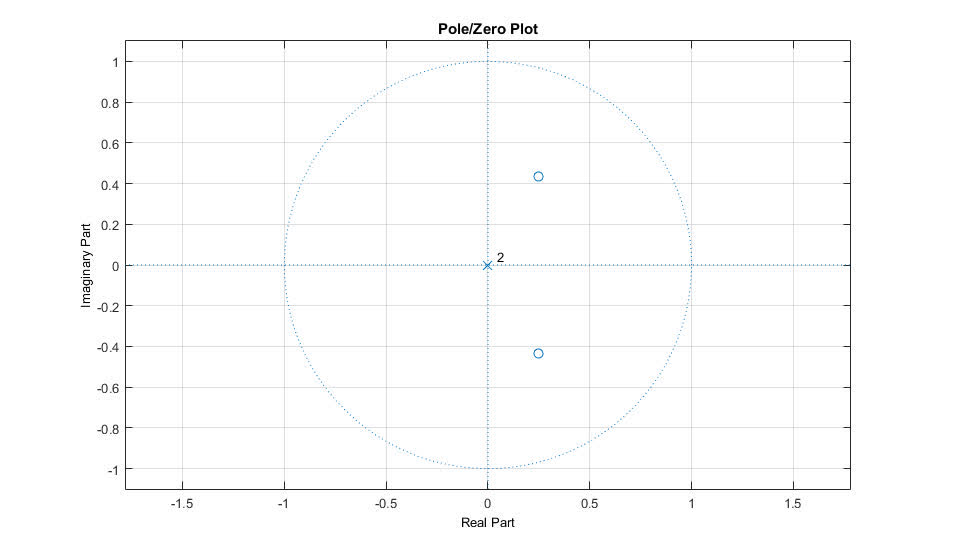
\includegraphics[width=1\textwidth]{images/20160223_02.png}
        \end{center}

        Magnitude is the same but with a different gain
        \begin{center}
            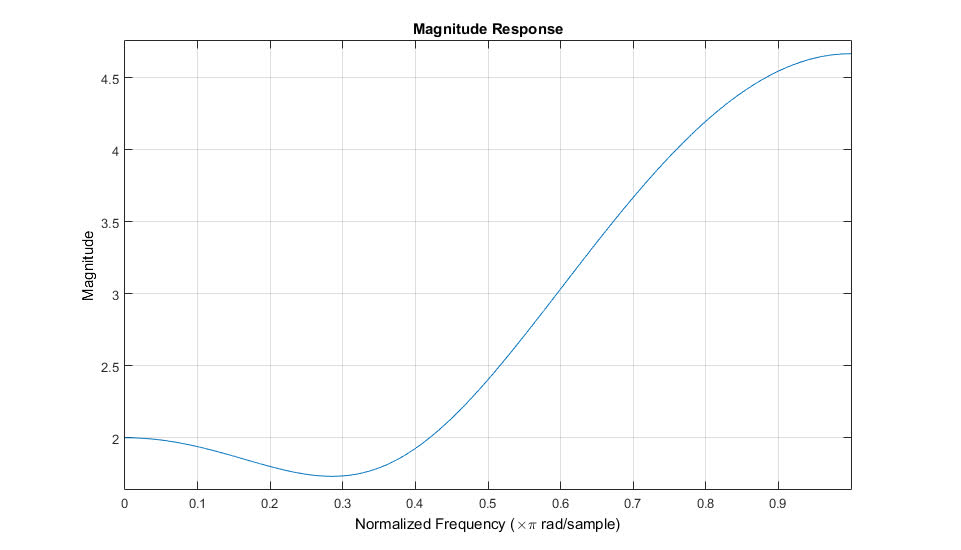
\includegraphics[width=1\textwidth]{images/20160223_03.png}
        \end{center}
    }

    \subsubsection{IIR filter to remove effect}
    Define a pure IIR filter $H_3(z)$ that, placed after the filter $H_2(z)$ is able to completely remove its effect

    \mybox{
        Remove the zeros
        $$
        H_3(z)=4\frac{1}{
            1-\frac{1}{2}z^{-1}+\frac{1}{4}z^{-2}
        }=4H_2(z)^{-1}
        $$
    }

    \subsubsection{Output samples}
    Find the first five output samples of the filters $H_1(z),H_2(z),H_3(z)$

    \mybox{
        $$
        x[n]=\delta[n]
        $$
        $$
        y_1[n]=x[n]-2x[n-1]+4x[n-2]
        $$
        So: \Brackets{1,-2,4}. For $y_2$ solve similarly. For $y_3$:
        $$
        y_3[n]=4\left(
            \frac{1}{2}y[n-1]-\frac{1}{4}y[n-2]
        \right)+x[n]
        $$
    }

\pagebreak\subsection{20160223-2}
    We want to remove the continuous component (zero frequency) from the periodic signal $x(n)$ represented below just working with the DFT.
    \begin{center}
        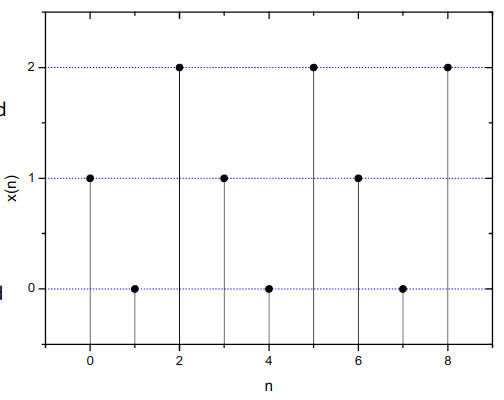
\includegraphics[width=0.7\textwidth]{images/20160223_05.png}
    \end{center}

    \subsubsection{DFT to remove continuous component}
    Propose a filter $H(k)$ in the frequency domain and apply it to the signal (provide also the $W$ matrix).

    \mybox{
        From the picture we can deduce:
        $$x(n)=\delta(n)+2\delta(n-2)$$
        With period 3. Reminder, the $W$ matrix is
        $$
        W=
        \begin{bmatrix}
            W_i^0 & W_i^0 & W_i^0 & W_i^0 & \cdots & W_i^n\\
            W_i^0 & W_i^1 & W_i^2 & W_i^3 & \cdots & W_i^{n-1}\\
            W_i^0 & W_i^2 & W_i^4 & W_i^6 & \cdots & W_i^{2(n-1)}\\
            W_i^0 & W_i^3 & W_i^6 & W_i^9 & \cdots & W_i^{3(n-1)}\\
            \vdots & \vdots & \vdots & \vdots & \ddots & \vdots\\
            W_i^0 & W_i^{n-1} & W_i^{2(n-1)} & W_i^{3(n-1)} & \cdots & W_i^{(n-1)^2}        
        \end{bmatrix}
        $$
        Where $W_i=e^{-j\frac{2\pi}{i}}$. In our case $i=3$
        $$W=
        \begin{bmatrix}
            1 & 1 & 1\\
            1 & -\frac{1}{2}-j\frac{\sqrt{3}}{2} & -\frac{1}{2}+j\frac{\sqrt{3}}{2}\\
            1 & -\frac{1}{2}+j\frac{\sqrt{3}}{2} & -\frac{1}{2}-j\frac{\sqrt{3}}{2}
        \end{bmatrix}
        $$
    }

    \mybox{
        So the DFT of x(n) will be:
        $$
        X(k)=
        \begin{bmatrix}
            1 & 1 & 1\\
            1 & -\frac{1}{2}-j\frac{\sqrt{3}}{2} & -\frac{1}{2}+j\frac{\sqrt{3}}{2}\\
            1 & -\frac{1}{2}+j\frac{\sqrt{3}}{2} & -\frac{1}{2}-j\frac{\sqrt{3}}{2}
        \end{bmatrix}
        \begin{bmatrix}
            1\\
            0\\
            2
        \end{bmatrix}=\begin{bmatrix}
            3\\
            \sqrt{3}j\\
            -\sqrt{3}j
        \end{bmatrix}
        $$
        As we want to remove the continuous component, we want to put 3 to 0 (the conjugates are 1 frequency), so we choose a
        $$H(k)=\begin{bmatrix}
            0\\
            1\\
            1
        \end{bmatrix}$$
        Applying it to the signal:
        $$Y(k)=X(k)\cdot H(k)=\begin{bmatrix}
            0\\
            \sqrt{3}j\\
            -\sqrt{3}j
        \end{bmatrix}$$
    }

    \subsubsection{DFT matrix inverse, output in time domain}
    Provide also the output in time domain $y(n)$ and a period of the filter in the time domain $h(n)$.

    \mybox{
        The inverse of $W$ is its conjugate transpose divided by $N=3$:
        $$
        W=
        \begin{bmatrix}
            1 & 1 & 1\\
            1 & -\frac{1}{2}-j\frac{\sqrt{3}}{2} & -\frac{1}{2}+j\frac{\sqrt{3}}{2}\\
            1 & -\frac{1}{2}+j\frac{\sqrt{3}}{2} & -\frac{1}{2}-j\frac{\sqrt{3}}{2}
        \end{bmatrix}
        \rightarrow
        W^{-1}=
        \frac{1}{3}
        \begin{bmatrix}
            1 & 1 & 1\\
            1 & -\frac{1}{2}+j\frac{\sqrt{3}}{2} & -\frac{1}{2}-j\frac{\sqrt{3}}{2}\\
            1 & -\frac{1}{2}-j\frac{\sqrt{3}}{2} & -\frac{1}{2}+j\frac{\sqrt{3}}{2}
        \end{bmatrix}
        $$
        $$
        y(n)=W^{-1}\cdot Y(k)=
        \frac{1}{3}
        \begin{bmatrix}
            1 & 1 & 1\\
            1 & -\frac{1}{2}+j\frac{\sqrt{3}}{2} & -\frac{1}{2}-j\frac{\sqrt{3}}{2}\\
            1 & -\frac{1}{2}-j\frac{\sqrt{3}}{2} & -\frac{1}{2}+j\frac{\sqrt{3}}{2}
        \end{bmatrix}
        \begin{bmatrix}
            0\\
            \sqrt{3}j\\
            -\sqrt{3}j
        \end{bmatrix}=
        \begin{bmatrix}
            0\\
            -1\\
            1
        \end{bmatrix}
        $$
        $$
        h(n)=W^{-1}\cdot H(k)=
        \frac{1}{3}
        \begin{bmatrix}
            1 & 1 & 1\\
            1 & -\frac{1}{2}+j\frac{\sqrt{3}}{2} & -\frac{1}{2}-j\frac{\sqrt{3}}{2}\\
            1 & -\frac{1}{2}-j\frac{\sqrt{3}}{2} & -\frac{1}{2}+j\frac{\sqrt{3}}{2}
        \end{bmatrix}
        \begin{bmatrix}
            0\\
            1\\
            1
        \end{bmatrix}=
        \begin{bmatrix}
            0\\
            -1/3\\
            -1/3
        \end{bmatrix}
        $$
    }

\pagebreak\subsection{20110202-1}
    Consider a signal made of infinite repertition of the following 4 samples: $\brackets{0;1;2;3}$

    \subsubsection{DFT}
    [4pts] Define the DFT matrix and provide the 4 Fourier coefficients for this signal

    \mybox{
        $$
        W_4=e^{-j\frac{2\pi}{4}}=e^{-j\frac{\pi}{2}}
        $$
        $$
        W=\begin{bmatrix}
            W_4^0 & W_4^0 & W_4^0 & W_4^0\\
            W_4^0 & W_4^1 & W_4^2 & W_4^3\\
            W_4^0 & W_4^2 & W_4^4 & W_4^6\\
            W_4^0 & W_4^3 & W_4^6 & W_4^9
        \end{bmatrix}=
        \begin{bmatrix}
            1 & 1 & 1 & 1\\
            1 &-j &-1 & j\\
            1 &-1 & 1 &-1\\
            1 & j &-1 &-j
        \end{bmatrix}
        $$
        $$
        X(k)=Wx=
        \begin{bmatrix}
            1 & 1 & 1 & 1\\
            1 &-j &-1 & j\\
            1 &-1 & 1 &-1\\
            1 & j &-1 &-j
        \end{bmatrix}
        \begin{bmatrix}
            0\\
            1\\
            2\\
            3
        \end{bmatrix}=
        \begin{bmatrix}
            6\\
            -2+2j\\
            -2\\
            -2-2j
        \end{bmatrix}
        $$
    }

    \subsubsection{Output samples: convolution}
    [4pts] An high pass filter, whose z-transform is $1-z^{-1}$ is applied to the signal, what will be the samples of the fitlered signal?

    \mybox{
        $$
        h[n]=\delta[n]-\delta[n-1]
        $$
        \textbf{Careful, the signal is PERIODIC, so}
        $$
        x[n-1]=\Brackets{3;0;1;2;3}
        $$
        And
        $$
        x[n]*h[n]=\Brackets{-3;1;1;1;-3}
        $$
    }

    \subsubsection{DFT}
    [4pts] What will be the DFT of the final signal?

    \mybox{
        $$
        \begin{bmatrix}
            1 & 1 & 1 & 1\\
            1 &-j &-1 & j\\
            1 &-1 & 1 &-1\\
            1 & j &-1 &-j
        \end{bmatrix}
        \begin{bmatrix}
            -3\\
            1\\
            1\\
            1
        \end{bmatrix}=
        \begin{bmatrix}
            0\\
            -4\\
            -4\\
            -4
        \end{bmatrix}
        $$
        Or compute the DFT of the filter $h$ and then multiply element-wise $y$ and $h$
    }
\end{document}